%\documentclass[english,xcolor=dvipsnames,bigger]{beamer}
\usepackage[sort&compress]{natbib}
\usepackage{tikz} 
\usepackage{mathptmx}
\usepackage{marvosym}
\usepackage[T1]{fontenc}
%\usepackage[latin1]{inputenc}
\usepackage{color}
\usepackage{amsmath}
\usepackage{amssymb}
\usepackage{tipa}

\only<beamer|trans|handout|draft>{
\newcommand{\newblock}{}
}

\usepackage{listings}
\usepackage{clrscode}

%%%%%%%%%% Farseerfc: fix the bug of xetex on navigation bar of beamer %%%%%%%%%

%\def\beamer@linkspace#1{%
%  \begin{pgfpicture}{0pt}{-1.5pt}{#1}{5.5pt}
%    \pgfsetfillopacity{0}
%    \pgftext[x=0pt,y=-1.5pt]{.}
%    \pgftext[x=#1,y=5.5pt]{.}
%  \end{pgfpicture}}

%%%%%%%%%% Farseerfc: fix the bug of xetex on navigation bar of beamer %%%%%%%%%

\usetheme{Madrid}
%\usecolortheme[named=OliveGreen]{structure}
%\setbeamercovered{dynamic}
\useoutertheme{infolines}
\usefonttheme{serif}
\usepackage[english]{babel}


\graphicspath{{figure/}}
\begin{document}

%%%%%%%%%%%%%%%%%%%%%%%%%%%%%%%%%%%%%%%%%%%%%%%%%%%%%%%%%%%%%%%%%%%%%%%%%%%%%%%%
% Farseerfc defined commands

\newcommand{\br}[0]{\par\vskip15pt\par}
%\newenvironment{topcolumns}{\begin{columns}[t]}{\end{columns}}

%%%%%%%%%%%%%%%%%%%%%%%%%%%%%%%%%%%%%%%%%%%%%%%%%%%%%%%%%%%%%%%%%%%%%%%%%%%%%%%%



\title[SuffixTree]{Algorithm of Suffix Tree}

\subtitle{by farseerfc@gmail.com}

\author[jc-yang]{
	Jiachen Yang\inst{1} 
}

\institute[Osaka-U]{
	\inst{1}Research Student in Osaka University
}



\frame{\maketitle}


\AtBeginSubsection[]{
  \frame<beamer>{ 
    \frametitle{Section Outline}   
    \tableofcontents[currentsection,currentsubsection] 
  }
}

\AtBeginSection[]{
  \frame<beamer>{ 
    \frametitle{Part Outline}   
    \tableofcontents[currentpart,currentsection] 
  }
}

\AtBeginPart{
  \frame<beamer>{
	\partpage
  }
}

%%%%%%%%%%%%%%%%%%%%%%%%%%%%%%%%%%%%%%%%%%%%%%%%%%%%%%%%%%%%%%%%%%%%%%%%%%%%%%%%
\section{What is Suffix Tree} 
\begin{frame}[shrink=25]{What can we do with suffix tree?}
\begin{columns}
\column{0.4\textwidth}
\alert{Linear algorithms} for exact string matching
\begin{itemize}
\item like KMP
\end{itemize}

Search for strings
\begin{enumerate}
\item   Check if a string $P$ of length $m$ is a substring in $O(m)$ time.
\item   Find all $z$ occurrences of the patterns $P_1,\cdots,P_q$ of total 
length $m$ as substrings in $O(m + z)$ time.
\item   Search for a regular expression $P$ in time expected sublinear in $n$ .
\item   Find for each suffix of a pattern $P$, the length of the longest match 
between a prefix of $P[i\ldots m]$ and a substring in $D$ in $\theta(m)$ time .
\item \dots
\end{enumerate}

\column{0.55\textwidth}
Find properties of the strings
\begin{enumerate}
\item   Find the longest common substrings of the string $S_i$ and $S_j$ 
in $\theta(n_i + n_j)$ time .
\item   \alert{Find all maximal pairs, maximal repeats or supermaximal repeats
 in $\theta(n + z)$ time, if there are $z$ such repeats .}
\item   Find the Lempel-Ziv decomposition in $\theta(n)$ time .
\item   Find the longest repeated substrings in $\theta(n)$ time.
\item   Find the most frequently occurring substrings of a minimum length in 
$\theta(n)$ time.
\item   Find the shortest strings from $\sum$ that do not occur in $D$, in 
$O(n + z)$ time, if there are $z$ such strings.
\item   Find the shortest substrings occurring only once in $\theta(n)$ time.
\item   Find, for each $i$, the shortest substrings of $S_i$ not occurring 
elsewhere in $D$ in $\theta(n)$ time.
\item \dots
\end{enumerate}
\end{columns}
\end{frame}
%%%%%%%%%%%%%%%%%%%%%%%%%%%%%%%%%%%%%%%%%%%%%%%%%%%%%%%%%%%%%%%%%%%%%%%%%%%%%%%%

\begin{frame}{Trie, Radix Tree, Suffix Trie \& Suffix Tree}
\begin{description}
\item[trie\footnote{pronounced as in word re\alert{trie}val by its 
inventor, \textipa{/tri:/} ``tree'', but pronounced \textipa{/traI/}
``try'' by other authors}] {\tiny (AKA prefix tree)} is a dictionary tree.
\begin{itemize}
\item stores a set of words.
\item each node represents a character {\tiny except that root is empty string}.
\item words with common prefix share same parent nodes.
\item minimal \alert{deterministic finite automaton} {\tiny that accepts all words}.
\end{itemize}
\item[radix tree]  {\tiny (AKA patricia trie or radix trie)} is a trie with 
compressed chain of nodes.
\begin{itemize}
\item Each internal node has at least 2 children.
\end{itemize}
\item[suffix trie] is a trie which stores all suffix of a given string.
\item[suffix tree] is a suffix radix tree.
\begin{itemize}
\item that enables \alert{linear time} construction and \alert{fast}
algorithms of other problems on a string.
\end{itemize}
\end{description}
\end{frame}
%%%%%%%%%%%%%%%%%%%%%%%%%%%%%%%%%%%%%%%%%%%%%%%%%%%%%%%%%%%%%%%%%%%%%
\begin{frame}{Trie \& Radix Tree}
\begin{columns}
\column{0.45\textwidth}
\begin{block}{Trie of ``A to tea ted ten i in inn''}
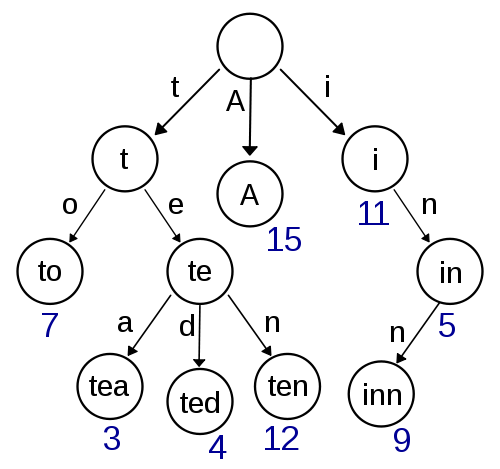
\includegraphics[width=\textwidth]{Trie_example.svg.png}
\end{block}
\column{0.5\textwidth}
\begin{block}{Radix tree example}
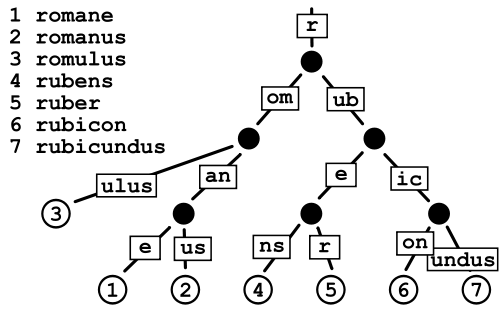
\includegraphics[width=\textwidth]{Patricia_trie.svg.png}
\end{block}
\end{columns}
\end{frame}

%%%%%%%%%%%%%%%%%%%%%%%%%%%%%%%%%%%%%%%%%%%%%%%%%%%%%%%%%%%%%%%%%%%%%
\begin{frame}{Suffix Trie \& Suffix Tree of ``banana''}
\begin{columns}
\column{0.45\textwidth}
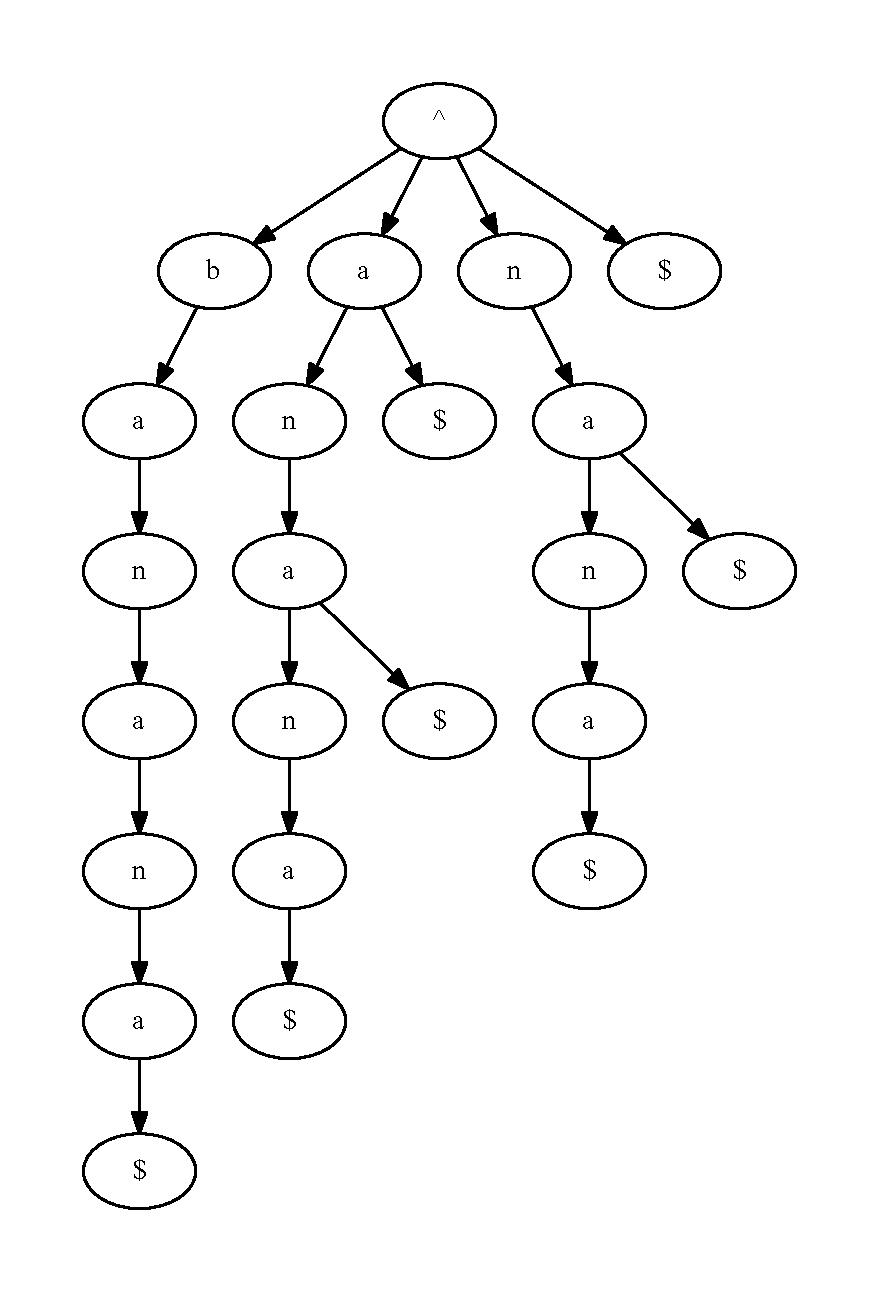
\includegraphics[height=0.8\textheight,trim=40pt 40pt 40pt 40pt]{banana-strie.pdf}
\column{0.5\textwidth}
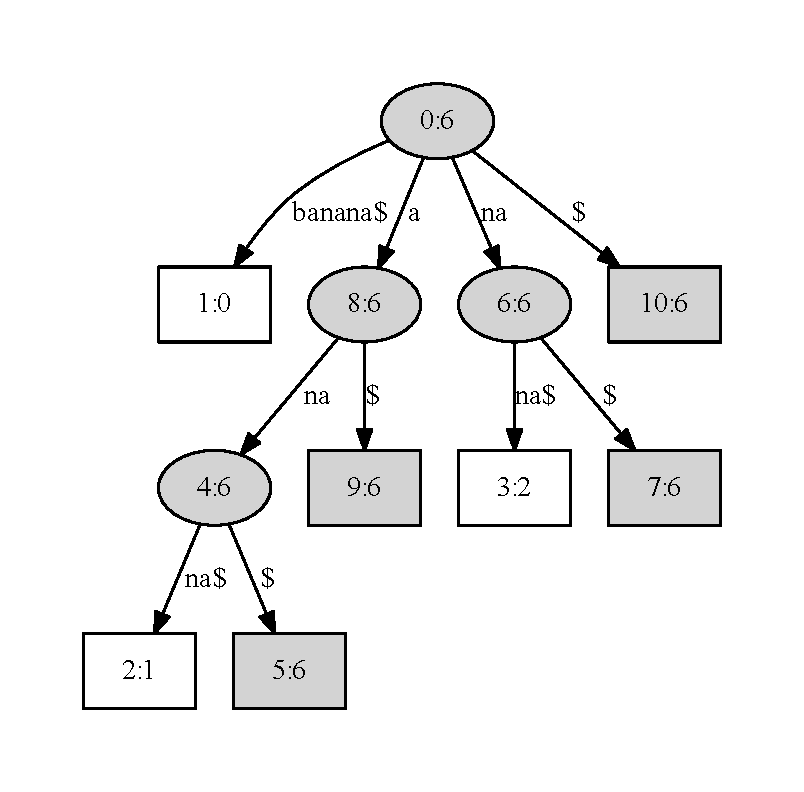
\includegraphics[width=0.9\textwidth,trim=40pt 40pt 40pt 40pt]{banana-st.pdf}
\end{columns}
\end{frame}
%%%%%%%%%%%%%%%%%%%%%%%%%%%%%%%%%%%%%%%%%%%%%%%%%%%%%%%%%%%%%%%%%%%%%

\begin{frame}{Suffix Tree of ``mississippi''}
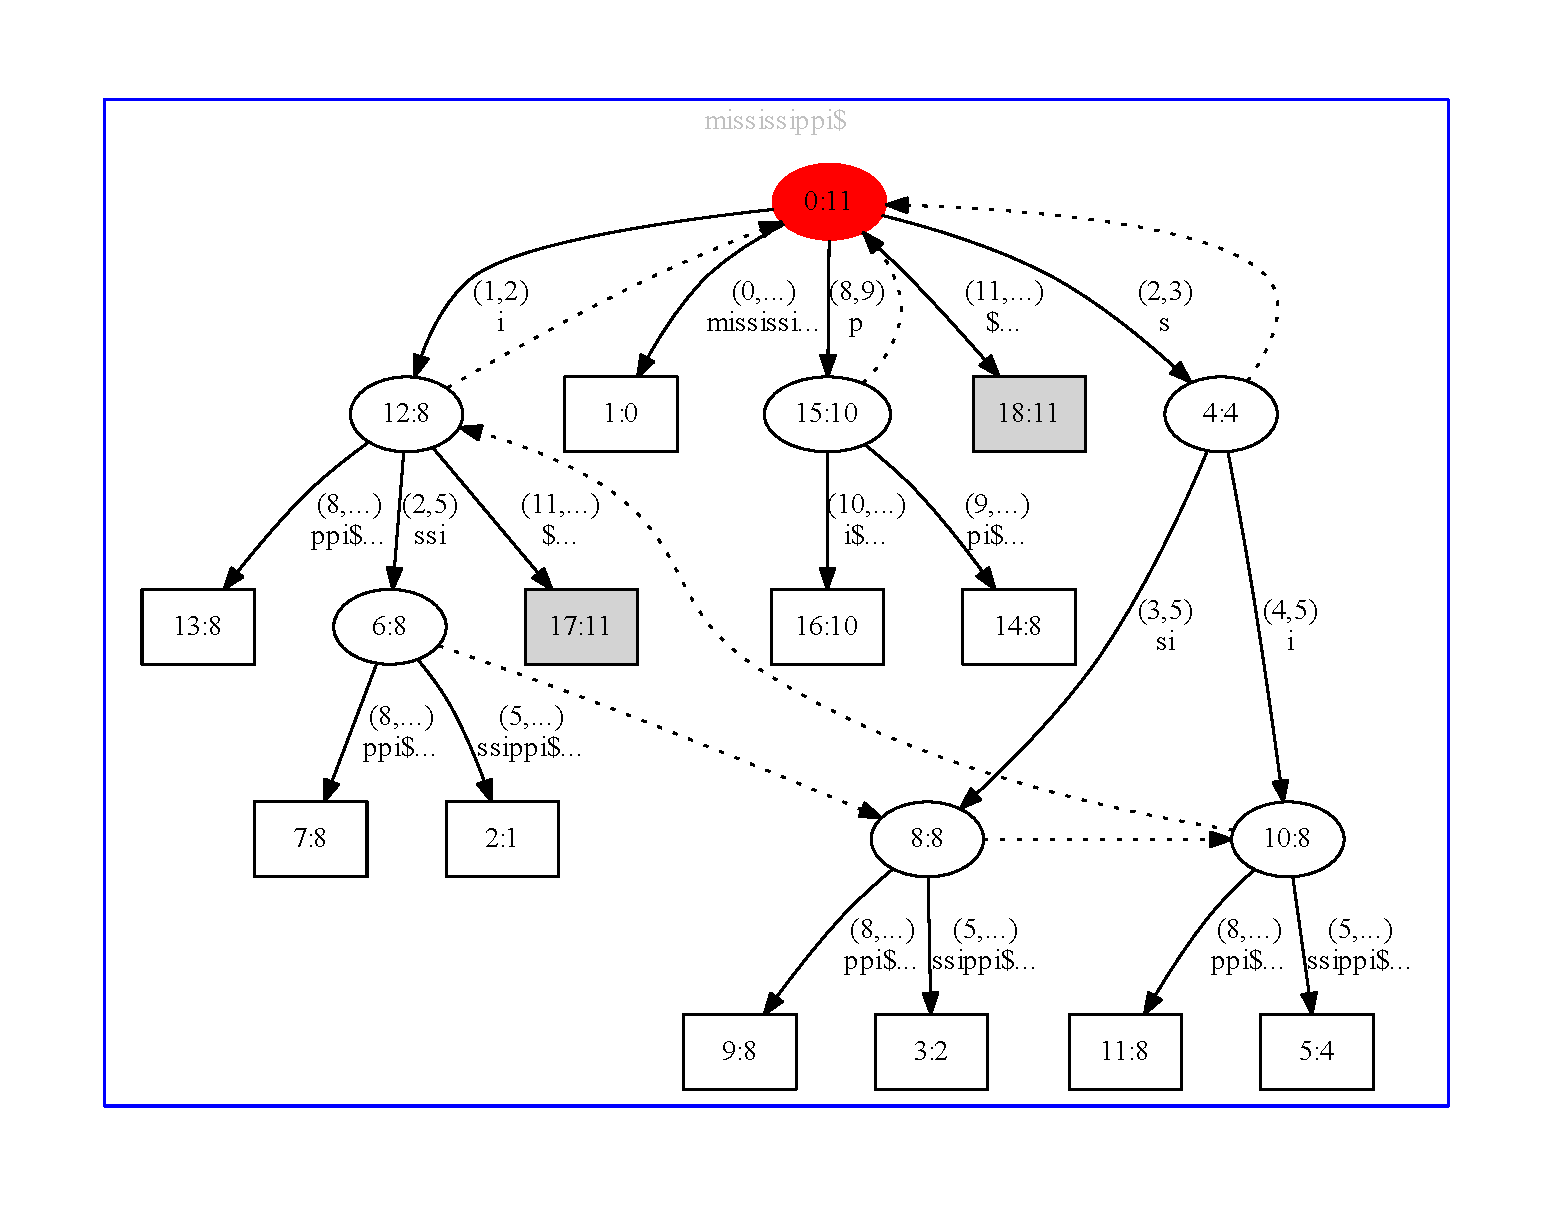
\includegraphics[height=0.8\textheight,trim=40pt 40pt 40pt 40pt]{mississippi_.pdf}
\end{frame}
%%%%%%%%%%%%%%%%%%%%%%%%%%%%%%%%%%%%%%%%%%%%%%%%%%%%%%%%%%%%%%%%%%%%%


\section{History \& Na\"{\i}ve Algorithm}

%%%%%%%%%%%%%%%%%%%%%%%%%%%%%%%%%%%%%%%%%%%%%%%%%%%%%%%%%%%%%%%%%%%%%
\begin{frame}[shrink=5]{History of Suffix Tree Algorithms}
\begin{columns}
\column{0.75\textwidth}
\begin{itemize}
\item First linear algorithm was introduced by \citealt{Wei73} as position
 tree. Awarded by Donald Knuth as ``Algorithm of the year 1973''.
\item Greatly simplified by \citealt{Mcc76}.
\end{itemize}

Above two algorithms are processing string \alert{backward}.

\begin{itemize}
\item First online construction by \citealt{Ukk95}, which is easier to understand.
\end{itemize}

Above algorithms assume size of \alert{alphabet as fixed} constant .

\begin{itemize}
\item Limitation was break by \citealt{farach97}, optimal for all alphabets.
\end{itemize}

Further study are continued to scale to scenarios when the whole suffix tree 
or even input string cannot fit into memory.
\column{0.22\textwidth}
{
\tiny
\bibliographystyle{abbrvnat}
\bibliography{ref}
}
\end{columns}
\end{frame}
%%%%%%%%%%%%%%%%%%%%%%%%%%%%%%%%%%%%%%%%%%%%%%%%%%%%%%%%%%%%%%%%%%%%%
\begin{frame}{Backward Construction of Suffix Tree}
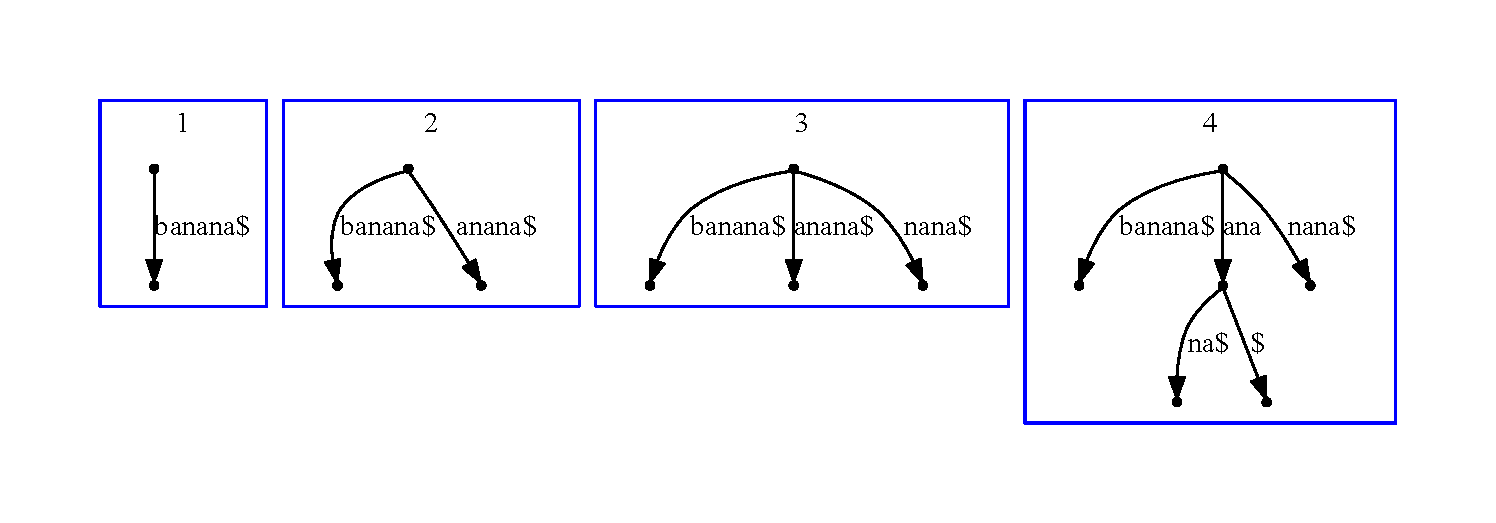
\includegraphics[height=0.32\textheight,trim=40pt 40pt 40pt 40pt]{back-banana_0-3.pdf}

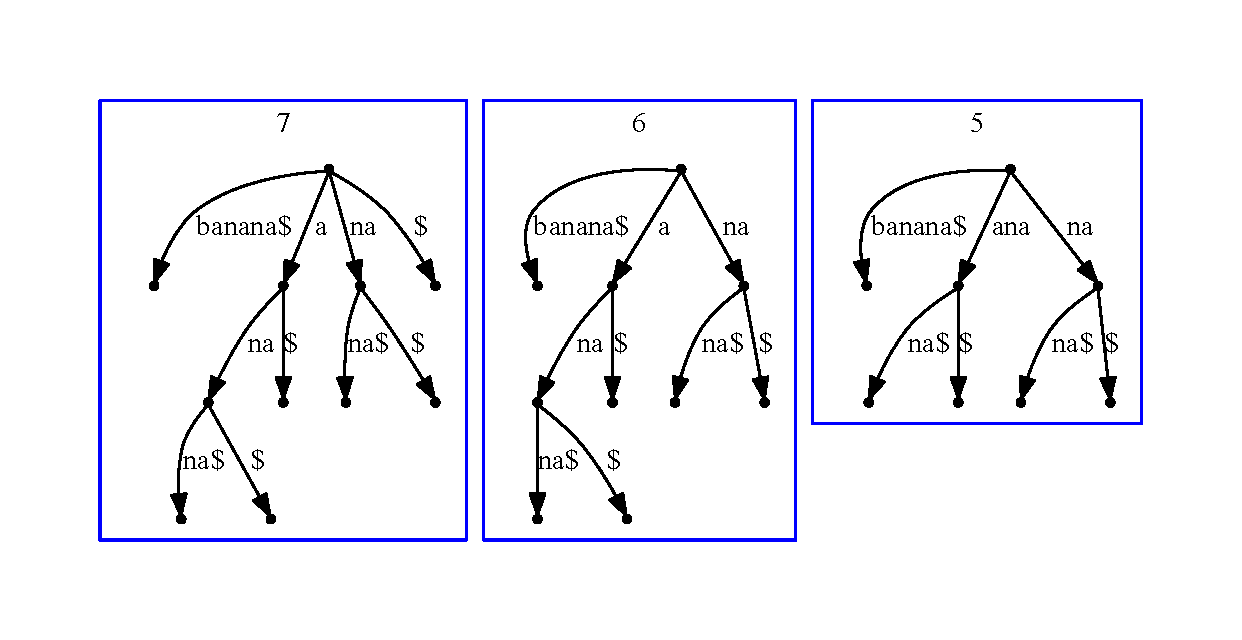
\includegraphics[height=0.52\textheight,trim=40pt 40pt 40pt 40pt]{back-banana_4-6.pdf}
\end{frame}


%%%%%%%%%%%%%%%%%%%%%%%%%%%%%%%%%%%%%%%%%%%%%%%%%%%%%%%%%%%%%%%%%%%%%

\begin{frame}[fragile]{Construct Suffix Tree by Sorting Suffix}

\lstset{basicstyle=\ttfamily}
\begin{columns}
\column{0.24\textwidth}
Suffix :
\begin{lstlisting}
mississippi
ississippi
ssissippi
sissippi
issippi
ssippi
sippi
ippi
ppi
pi
i
\end{lstlisting}
\column{0.24\textwidth}
Sorted suffix :
\begin{lstlisting}
i
ippi
issippi
ississippi
mississippi
pi
ppi
sippi
sissippi
ssippi
ssissippi
\end{lstlisting}

\column{0.44\textwidth}
Tree of sorted suffix :
\lstset{columns=fixed}
\begin{lstlisting}
|-i->|-
|    |-ppi 
|    |-ssi->|-ppi 
|           |-ssippi
|-mississippi 
|-p->|-i 
|    |-pi 
|-s->|-i-->|-ppi
     |     |-ssippi
     |-si->|-ppi
           |-ssippi
\end{lstlisting}
\end{columns}
Time complexity will be $O(N^2 \log N)$ .

Space complexity will be $O(N^2)$ .
\end{frame}


%%%%%%%%%%%%%%%%%%%%%%%%%%%%%%%%%%%%%%%%%%%%%%%%%%%%%%%%%%%%%%%%%%%%%
\begin{frame}{Na\"{\i}ve Algorithm }

\begin{codebox}
\Procname{$\proc{SuffixTree}(string)$}
\li \For $i \gets 1$ \To \textbf{length}$(string)$
\li     \Do $\proc{Update}(tree_i)$ \qquad \Comment Phrase i
        \End
\end{codebox}

\begin{codebox}
\Procname{$\proc{Update}(tree_i)$}
\li \For $j \gets 1$ \To $i$
\li     \Do $node \gets  tree_i.\proc{Find}(suffix[j$ \To $i-1])$
\li     $\proc{Extend}(node, string[i])$ \qquad \Comment Extension j
        \End
\end{codebox}

Time complexity will be $O(N^3)$ .

Space complexity will be $O(N^2)$ .

The challenge is to make sure $tree_i$ is updated to 
$tree_{i+1}$ \alert{efficiently}. 
\end{frame}


%%%%%%%%%%%%%%%%%%%%%%%%%%%%%%%%%%%%%%%%%%%%%%%%%%%%%%%%%%%%%%%%%%%%%
\begin{frame}[shrink=20]{Suffix Extend Cases of Na\"{\i}ve Algorithm}
\begin{description}
\item[Case I] If path $S_{j\ldots i}$ ends at leaf, append a char $S_{i+1}$
to end of edge into leaf.
\begin{columns}
\column{0.2\textwidth}
$S_{j\ldots i} = \ldots na$ 

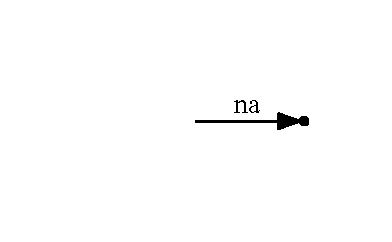
\includegraphics[trim=80pt 35pt 80pt 35pt]{na.pdf}
\column{0.1\textwidth}
{\huge \MVRightarrow}
\column{0.2\textwidth}
$S_{j\ldots i+1} = \ldots nan$ 

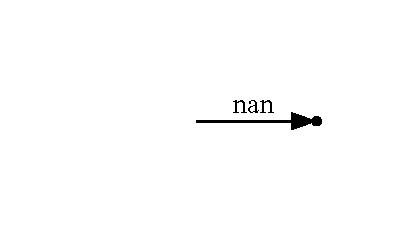
\includegraphics[trim=80pt 35pt 80pt 35pt]{nan.pdf}
\end{columns}
\item[Case II] If path $S_{j...i}$ ends in the middle of an edge ,
and next char $S_{i+1}$ is \alert{not equal} to the next char in the edge,
split that edge, create a internal node, add a new edge to a new leaf.
\begin{columns}
\column{0.2\textwidth}
$S_{j\ldots i} = \ldots na$ 

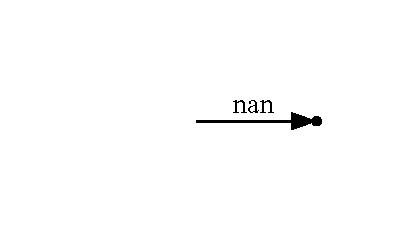
\includegraphics[trim=80pt 35pt 80pt 35pt]{nan.pdf}
\column{0.1\textwidth}
{\huge \MVRightarrow}
\column{0.2\textwidth}
$S_{j\ldots i+1} = \ldots nay$ 

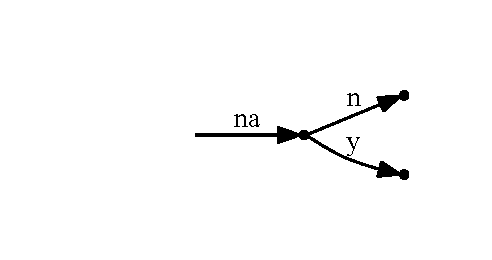
\includegraphics[trim=80pt 35pt 80pt 35pt]{nany.pdf}
\end{columns}
\item[Case III] If path $S_{j...i}$ ends in the middle of an edge ,
and next char $S_{i+1}$ is \alert{equal} to the next char in the edge,
do nothing, extenstion has done.
\begin{columns}
\column{0.2\textwidth}
$S_{j\ldots i} = \ldots na$ 

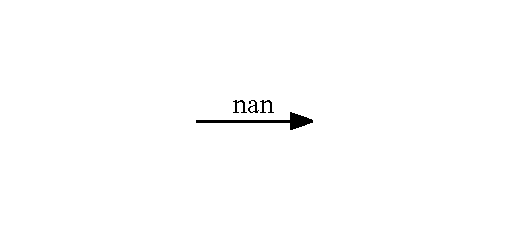
\includegraphics[trim=80pt 35pt 80pt 35pt]{nan_.pdf}
\column{0.1\textwidth}
{\huge \MVRightarrow}
\column{0.2\textwidth}
$S_{j\ldots i+1} = \ldots nan$ 

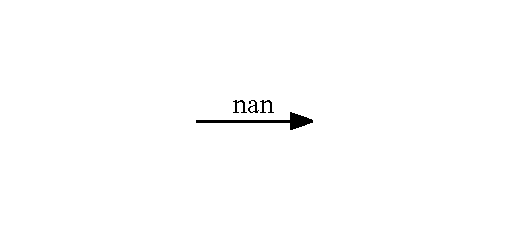
\includegraphics[trim=80pt 40pt 80pt 35pt]{nan_.pdf}
\end{columns}
\end{description}
\end{frame}

%%%%%%%%%%%%%%%%%%%%%%%%%%%%%%%%%%%%%%%%%%%%%%%%%%%%%%%%%%%%%%%%%%%%%
\begin{frame}{Na\"{\i}ve Online Construction of Suffix Tree}
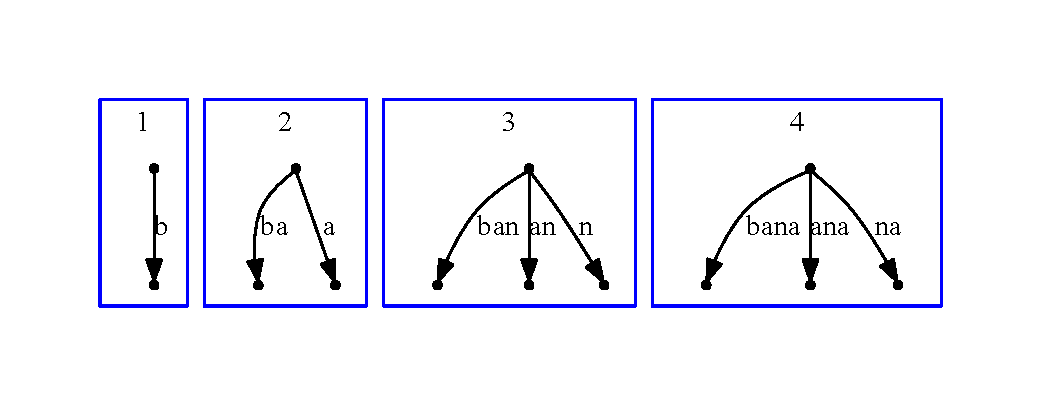
\includegraphics[height=0.35\textheight,trim=40pt 40pt 40pt 40pt]{naive-banana_0-3.pdf}

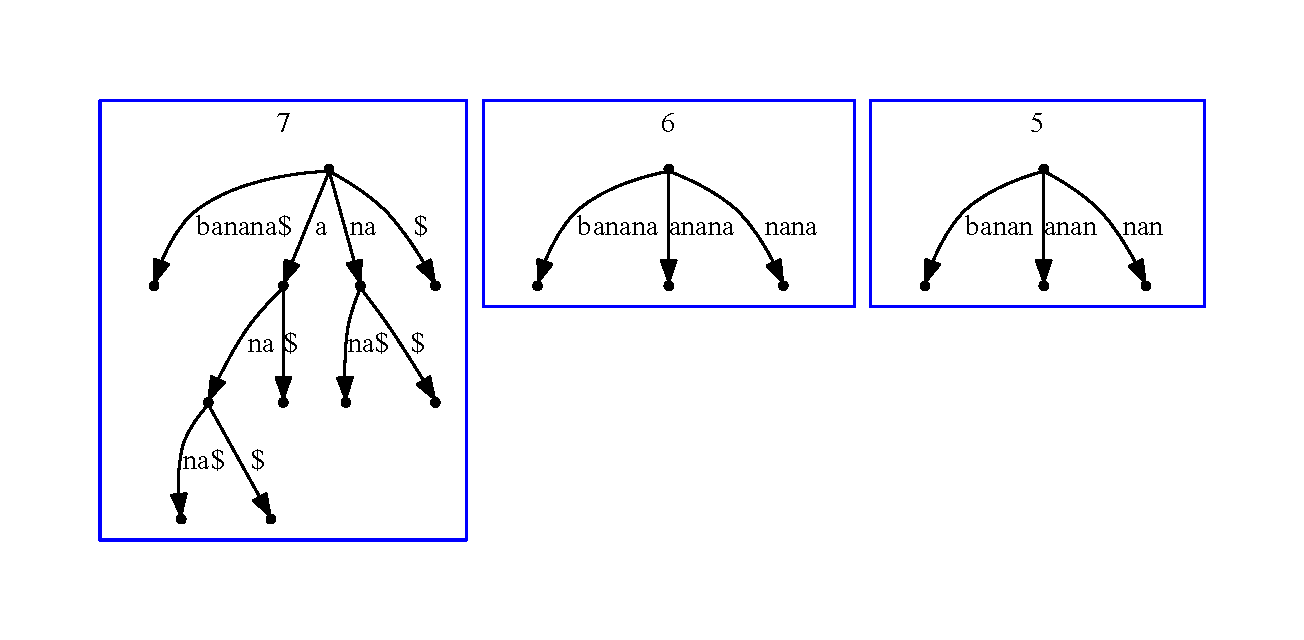
\includegraphics[height=0.51\textheight,trim=40pt 40pt 40pt 40pt]{naive-banana_4-6.pdf}
\end{frame}

%%%%%%%%%%%%%%%%%%%%%%%%%%%%%%%%%%%%%%%%%%%%%%%%%%%%%%%%%%%%%%%%%%%%%
\begin{frame}[shrink=10]{Properties of Suffix Tree}
\begin{columns}
\column{0.5\textwidth}
\begin{enumerate}
\item Each update will add exactly 1 leaf node .
\begin{itemize}
\item $nr\_leaf = N$
\end{itemize}
\item Suffix tree is full tree. 
\begin{itemize}
\item Each internal node has at least 2 children.
\item $nr\_internal < N$
\item $nr\_node < 2 N$
\end{itemize}
\item Worst case Fabonacci word 
\begin{itemize}
\item abaababaabaab
\end{itemize}
\item Suffix is either explicit or implicit.
\begin{itemize}
\item Explicit when it ends at a node.
\item Implicit when it ends in the middle of an edge.
\end{itemize}
\end{enumerate}
\column{0.45\textwidth}
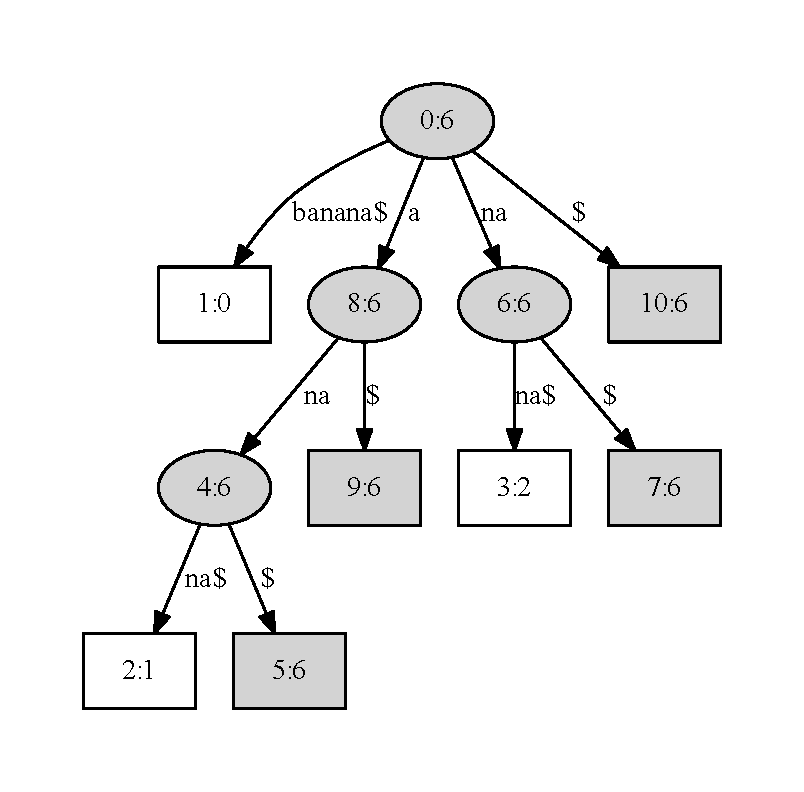
\includegraphics[width=\textwidth,trim=50pt 50pt 50pt 50pt]{banana-st.pdf}
\end{columns}

\end{frame}
%%%%%%%%%%%%%%%%%%%%%%%%%%%%%%%%%%%%%%%%%%%%%%%%%%%%%%%%%%%%%%%%%%%%%


\section{Optimization of Na\"{\i}ve Algorithm}


\begin{frame}[shrink=5]{Optimization of Na\"{\i}ve Algorithm}
\begin{enumerate}
\item Substrings can be represented as (start, end) pair of their index in orignal string.
\begin{itemize}
\item Reduce space complexity to \alert{$O(N)$} if size of alphabet is fixed constant.
\end{itemize}
\item Once a leaf, Always a leaf
\begin{itemize}
\item Represent edge that links to a leaf as (start, $\cdots$ ).
\item Extend leaf nodes \alert{for free}. We do not need Extend Case I.
\end{itemize}
\end{enumerate}
 
\begin{columns}
\column{0.40\textwidth}
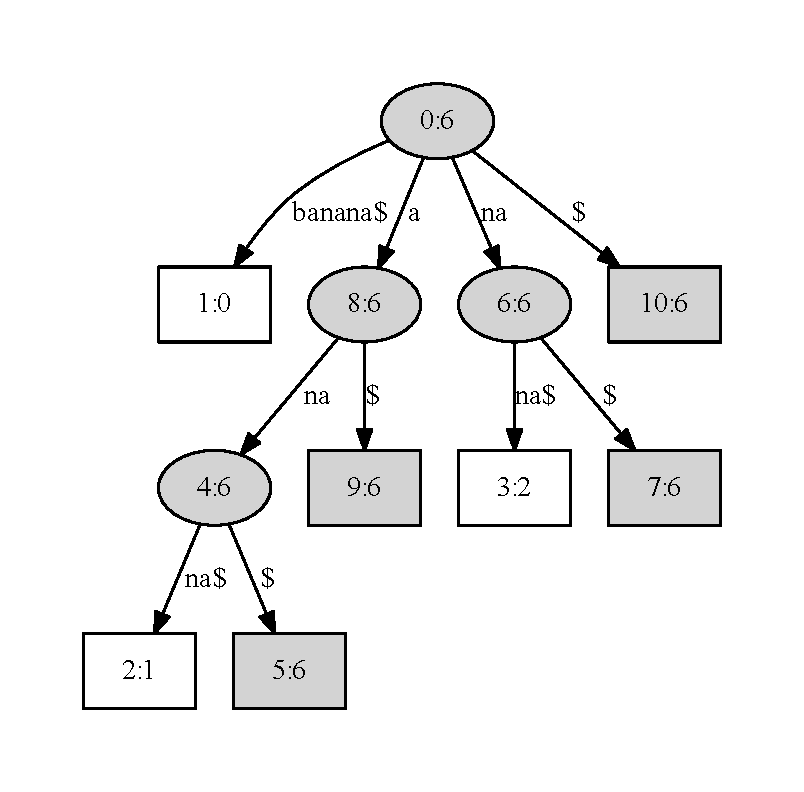
\includegraphics[width=\textwidth,trim=40pt 40pt 40pt 40pt]{banana-st.pdf}
\column{0.1\textwidth}
{\huge \MVRightarrow}
\column{0.45\textwidth}
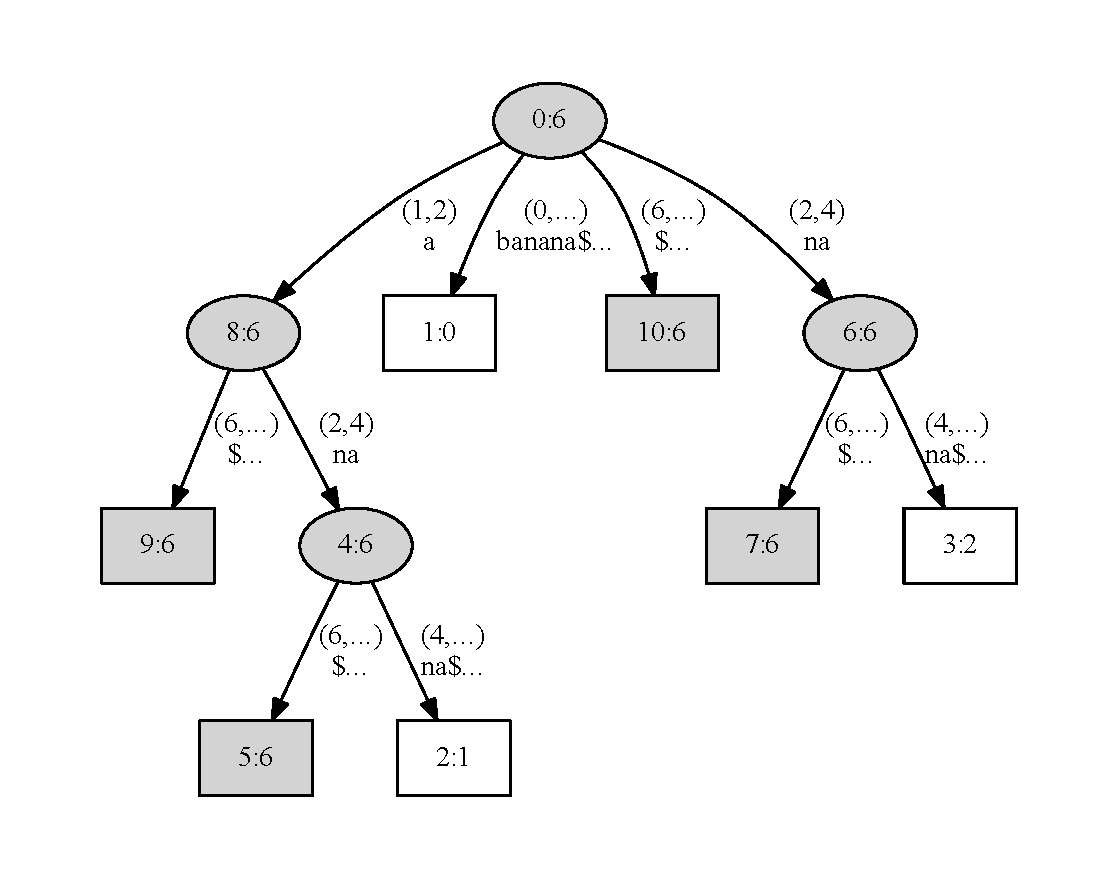
\includegraphics[width=\textwidth,trim=50pt 50pt 50pt 50pt]{banana_.pdf}
\end{columns}
\end{frame}
%%%%%%%%%%%%%%%%%%%%%%%%%%%%%%%%%%%%%%%%%%%%%%%%%%%%%%%%%%%%%%%%%%%%%

\begin{frame}{Active Point}
\begin{itemize}
\item During a phrase, if we meet Extend Case III, that is if we found 
$S[i+1]$ already exists in $suffix[j \ldots i]$ then $S[i+1]$ will exists
 in $\forall suffix[k \ldots i], k \in j \ldots i $.
\item Thus Case III is a sign that means update of this phrase is finished.

\item During phrase $i$ if we stopped at $suffix[k \ldots i]$ by Case III,
 then in next phrase we can start from $suffix[k \ldots i+1]$ because all suffix
start with $1 \ldots k-1$ will end at Case I.

\item We called this point(current internal node, current position $k$ in string) as \alert{Active Point}.
\end{itemize}
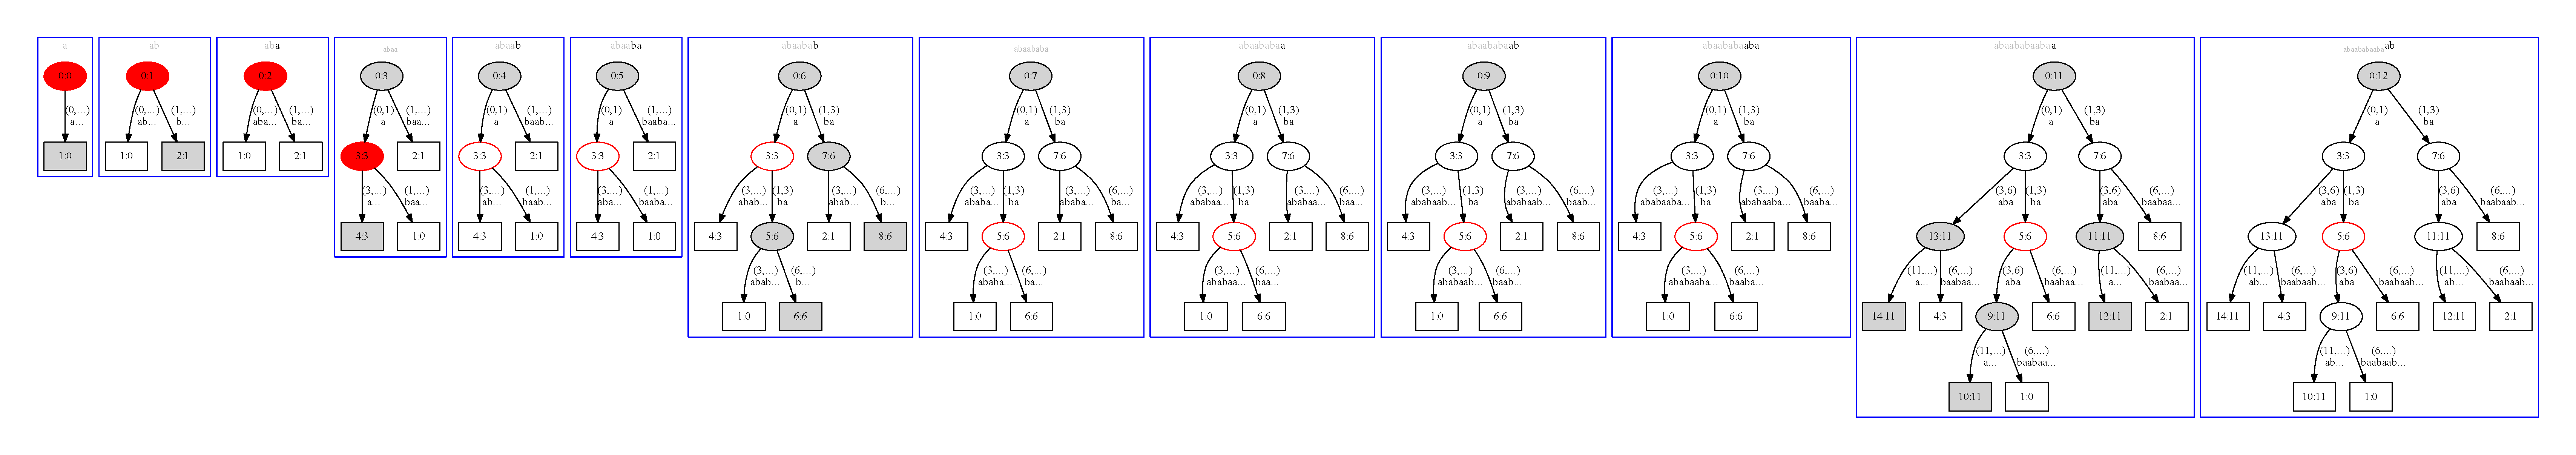
\includegraphics[width=\textwidth,trim=50pt 50pt 50pt 40pt]{abaababaabaab.pdf}
\end{frame}
%%%%%%%%%%%%%%%%%%%%%%%%%%%%%%%%%%%%%%%%%%%%%%%%%%%%%%%%%%%%%%%%%%%%%

\begin{frame}{Ukk's Update using Active Point}
\begin{codebox}
\Procname{$\proc{Update}(tree_i)$}
\li $current\_suffix \gets active\_point$
\li $next\_char \gets string[i] $
\li \While \textbf{True}
\li  \Do 
       \If there exists edge start with $next\_char$
\li          \Then \textbf{break} \qquad \Comment Case III
\li          \Else
\li               split current edge if implicit
\li               create new leaf with new edge labelled $next\_char$
             \End
\li   \If $current\_suffix$ is empty
\li   \Then  \textbf{break}
\li   \Else  $current\_suffix \gets$ \alert{next shorter suffix}
      \End
    \End
\li $active\_point \gets current\_suffix$
\end{codebox}

\end{frame}

%%%%%%%%%%%%%%%%%%%%%%%%%%%%%%%%%%%%%%%%%%%%%%%%%%%%%%%%%%%%%%%%%%%%%

\begin{frame}{Suffix Link to find next shorter suffix}
\begin{itemize}
\item Suffix link
\begin{itemize}
\item Internal node of suffix $X\alpha$ has a link to node $\alpha$.
\item If $\alpha$ is empty, suffix link points to root.
\end{itemize}
\item How to create suffix link
\begin{itemize}
\item Link together every internal nodes that are created by splitting in same phrase.
\end{itemize}
\end{itemize}

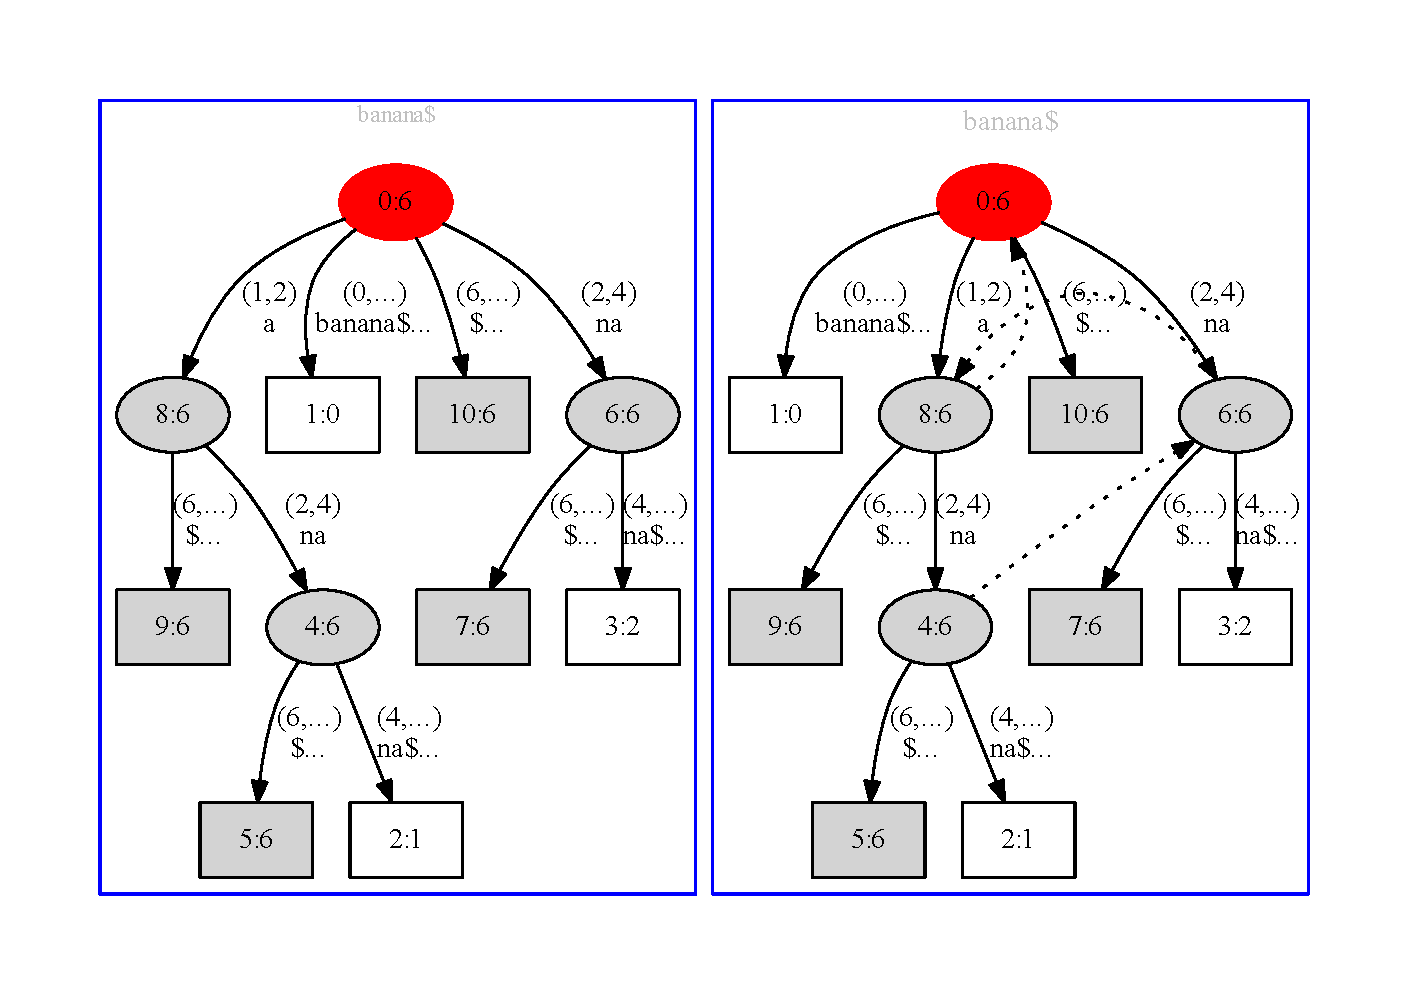
\includegraphics[width=0.6\textwidth,trim=50pt 50pt 50pt 40pt]{sl-banana_.pdf}
\end{frame}
%%%%%%%%%%%%%%%%%%%%%%%%%%%%%%%%%%%%%%%%%%%%%%%%%%%%%%%%%%%%%%%%%%%%%
\begin{frame}{Fast jump using Suffix Link}
\begin{itemize}
\item Assume we are at Suffix $X\alpha\beta$, whose parent internal node represent
$X\alpha$. 
\begin{enumerate}
\item Go back to parent internal node,
\item Jumping follow the node's suffix link to the node represent Suffix $\alpha$
\item Go down to Suffix $\alpha\beta$.
\end{enumerate}
\item Even jump down in step 3 because we already know length of $\beta$. (Skip/Count trick)
\item Combining all these tricks we can Extend a character in \alert{$O(1)$} time.
\end{itemize}
\end{frame}

%\begin{frame}{Algorithm of Constructing Suffix Tree}%
%\begin{columns}%
%\transfade[duration=0.2]<2->
%\column{0.5\textwidth}
%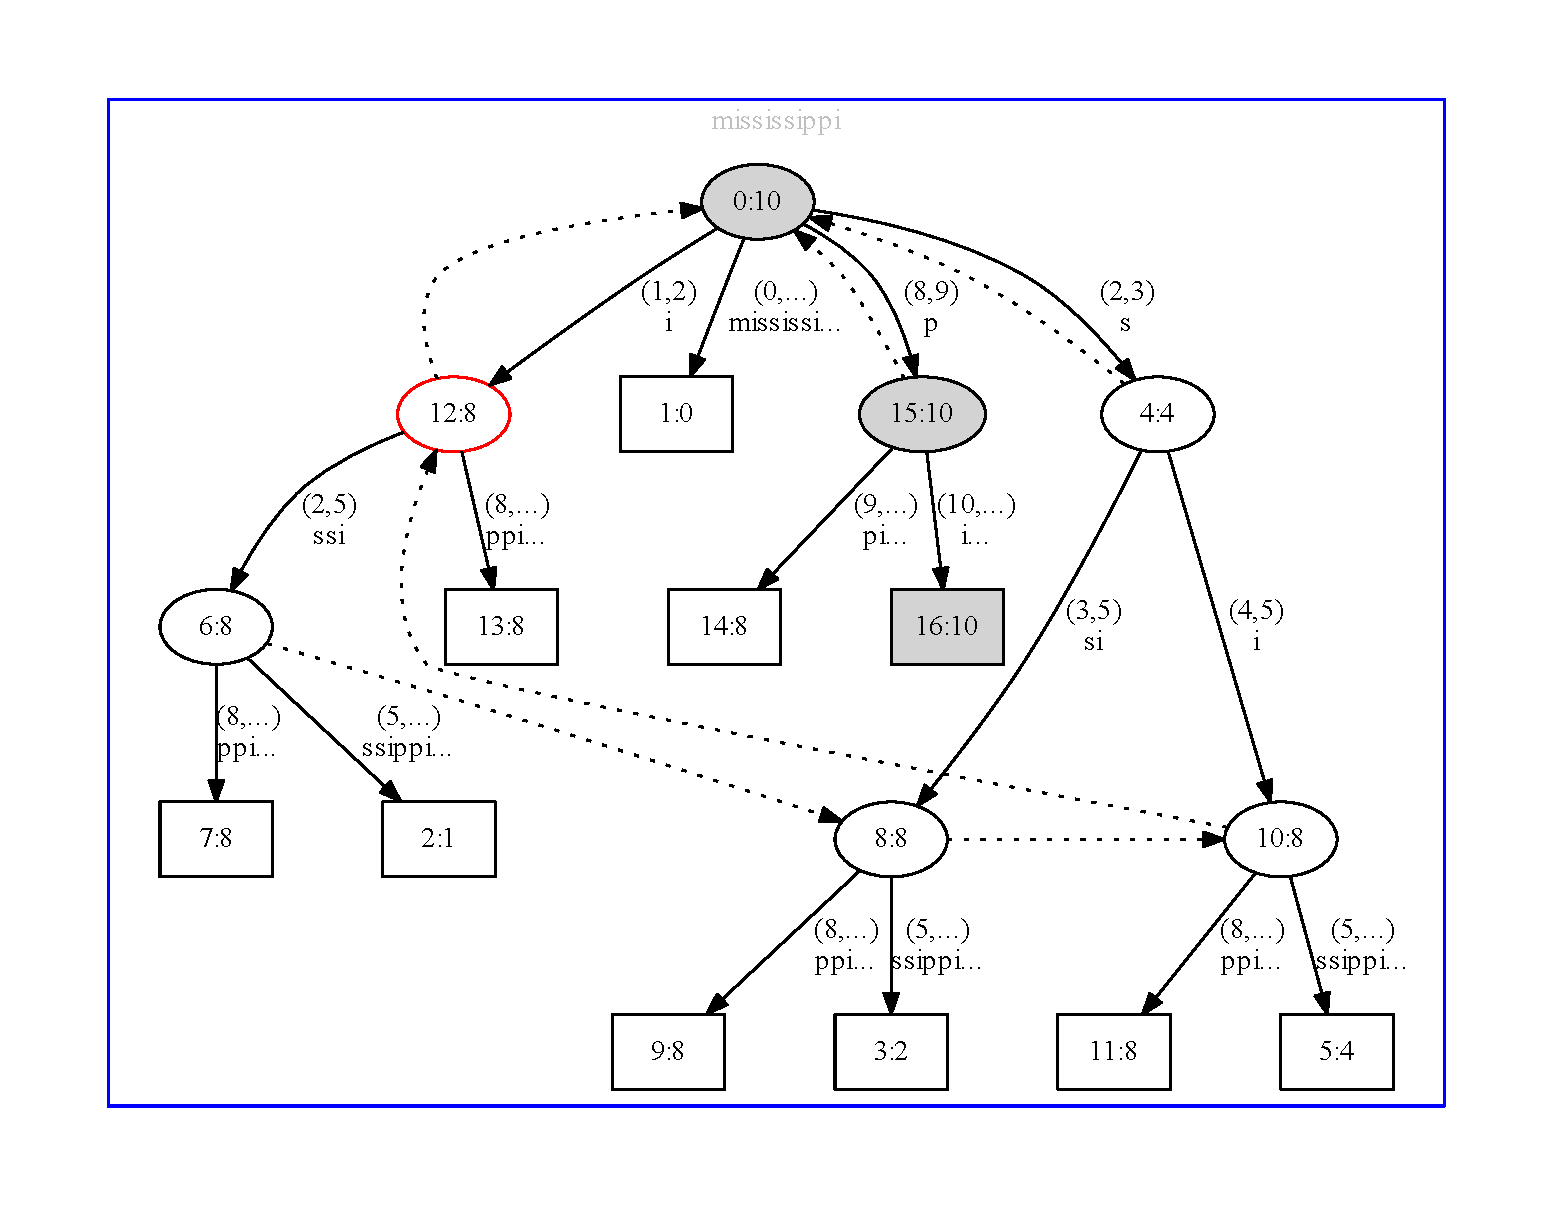
\includegraphics[width=\textwidth,trim=40pt 40pt 40pt 40pt]{mississippi.pdf}
%
%\column{0.45\textwidth}
%\begin{itemize}
%\item<2-> 
%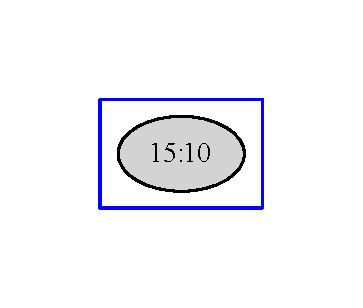
\includegraphics[width=0.25\textwidth,trim=40pt 40pt 40pt 40pt]{gray.pdf} 
%Node (id:generation)
%\item<3-> 
%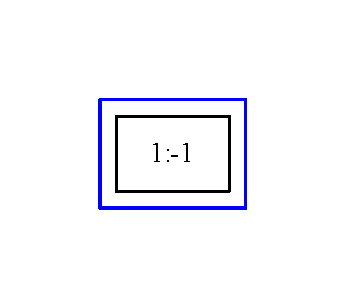
\includegraphics[width=0.25\textwidth,trim=40pt 40pt 40pt 40pt]{box.pdf} 
%Leaf
%\item<4-> 
%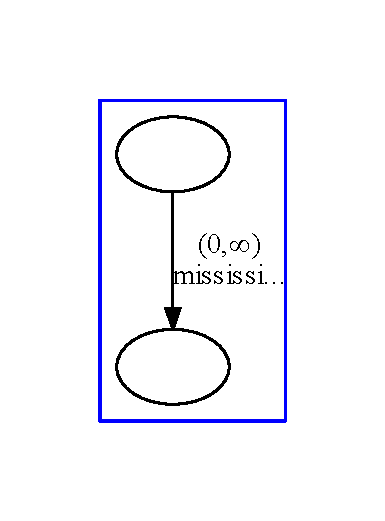
\includegraphics[width=0.25\textwidth,trim=40pt 40pt 40pt 40pt]{line.pdf} 
%Child-relation
%\item<5-> 
%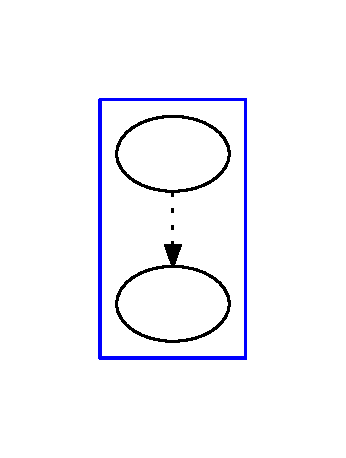
\includegraphics[width=0.25\textwidth,trim=40pt 40pt 40pt 40pt]{dotted.pdf} 
%suffix-link relation
%\end{itemize}
%\end{columns}
%\end{frame}

%%%%%%%%%%%%%%%%%%%%%%%%%%%%%%%%%%%%%%%%%%%%%%%%%%%%%%%%%%%%%%%%%%%%%%%%%%%%%%%%
\section{Examples \& Analysis}
\begin{frame}[shrink=13]{Experiment -- mississippi}

\transfade[duration=0.1]<2->
\begin{overlayarea}{\textwidth}{\textheight}
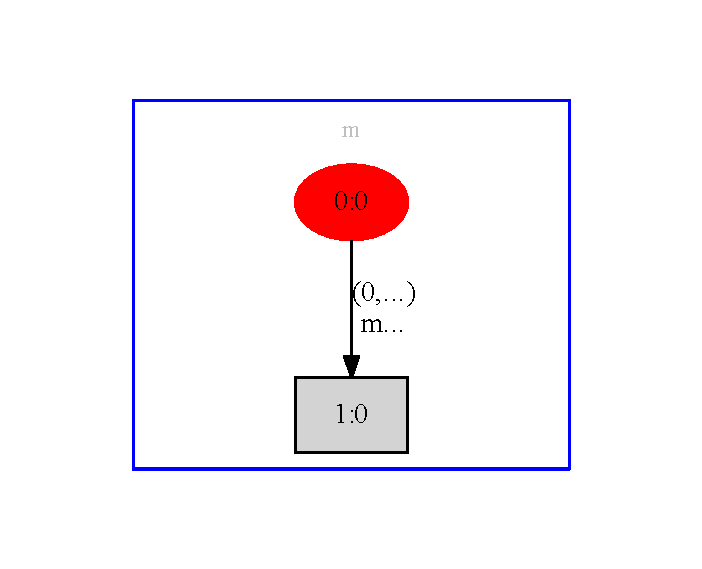
\includegraphics[keepaspectratio,trim=40pt 40pt 40pt 40pt,height=0.8\textheight,width=0.9\textwidth]{m.pdf}<1>
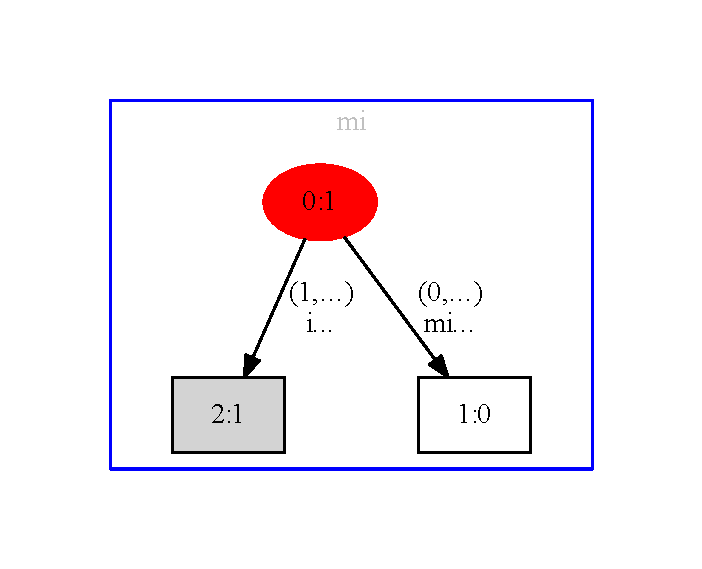
\includegraphics[keepaspectratio,trim=40pt 40pt 40pt 40pt,height=0.8\textheight,width=0.9\textwidth]{mi.pdf}<2>
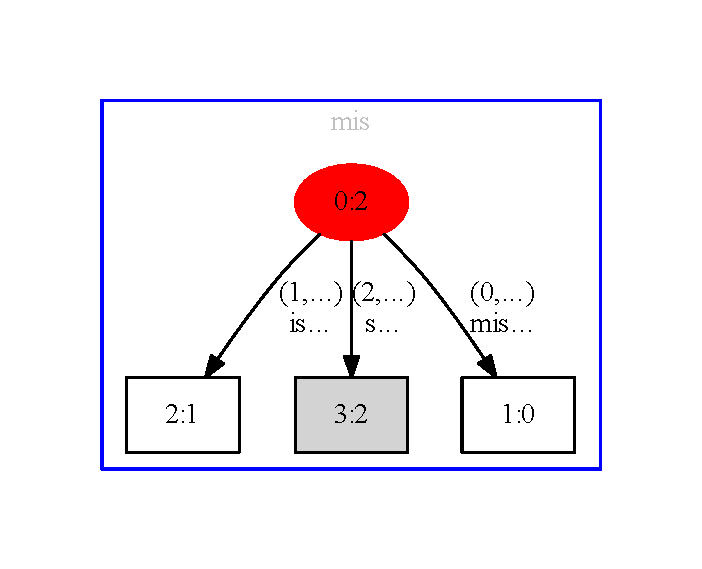
\includegraphics[keepaspectratio,trim=40pt 40pt 40pt 40pt,height=0.8\textheight,width=0.9\textwidth]{mis.pdf}<3>
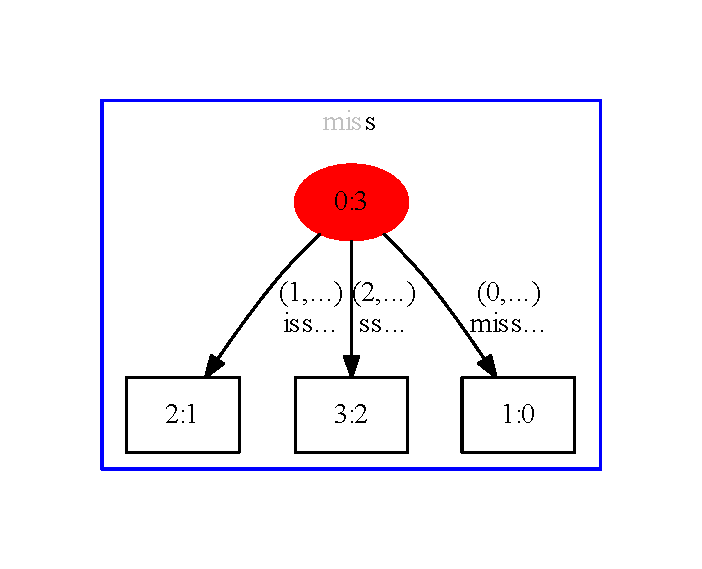
\includegraphics[keepaspectratio,trim=40pt 40pt 40pt 40pt,height=0.8\textheight,width=0.9\textwidth]{miss.pdf}<4>
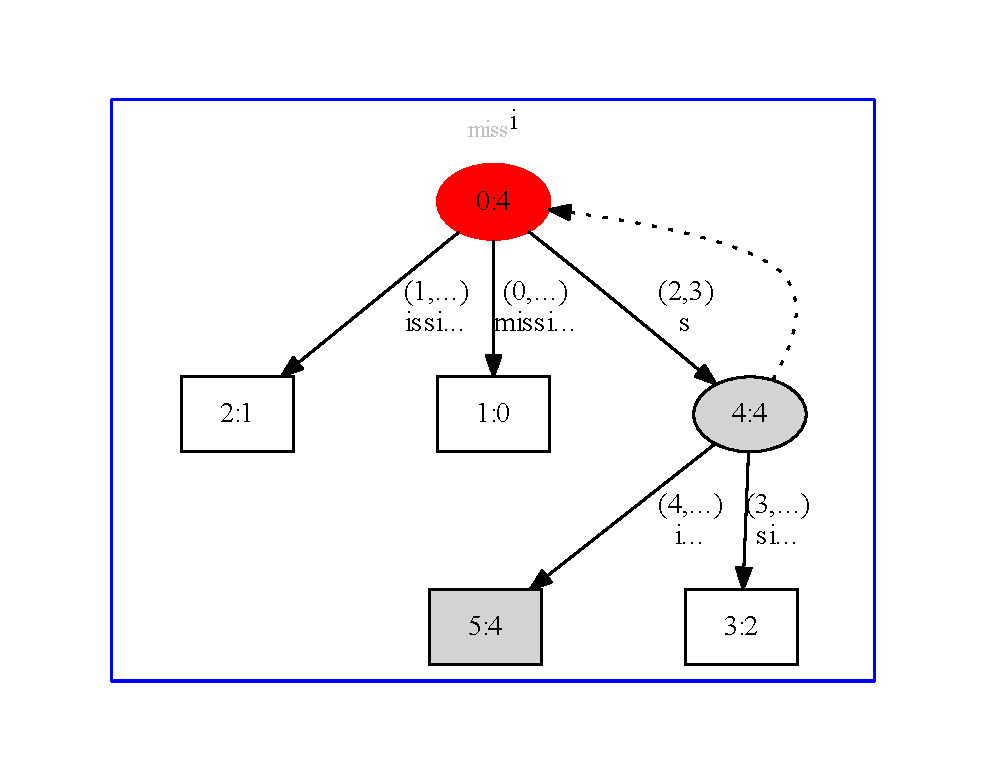
\includegraphics[keepaspectratio,trim=40pt 40pt 40pt 40pt,height=0.8\textheight,width=0.9\textwidth]{missi.pdf}<5>
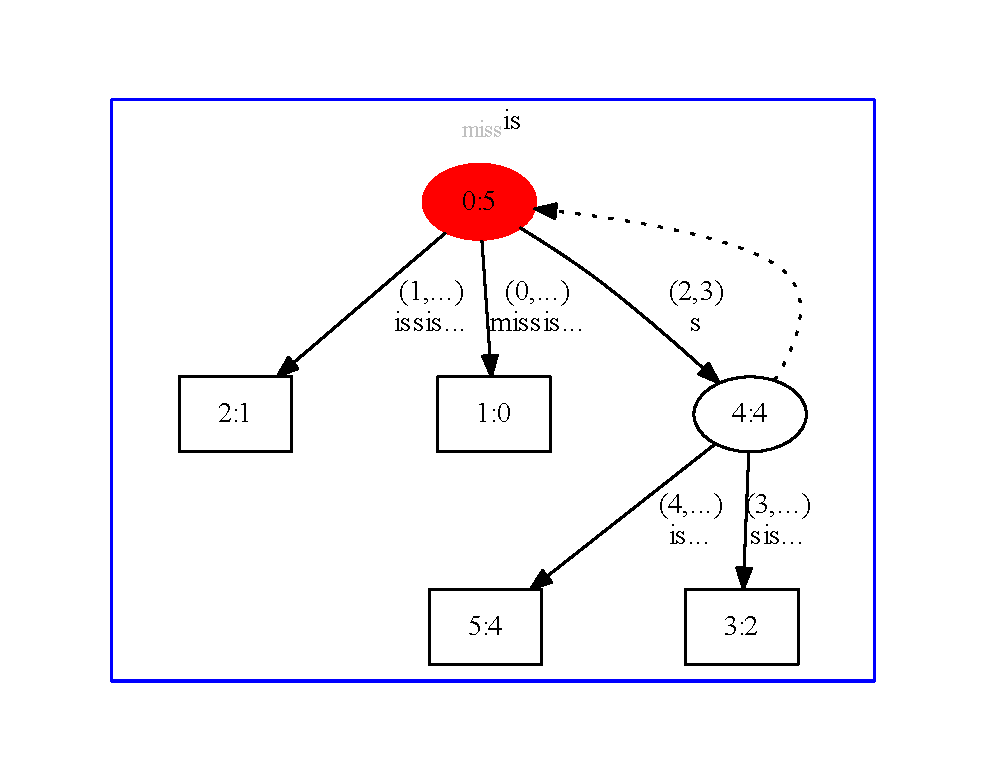
\includegraphics[keepaspectratio,trim=40pt 40pt 40pt 40pt,height=0.8\textheight,width=0.9\textwidth]{missis.pdf}<6>
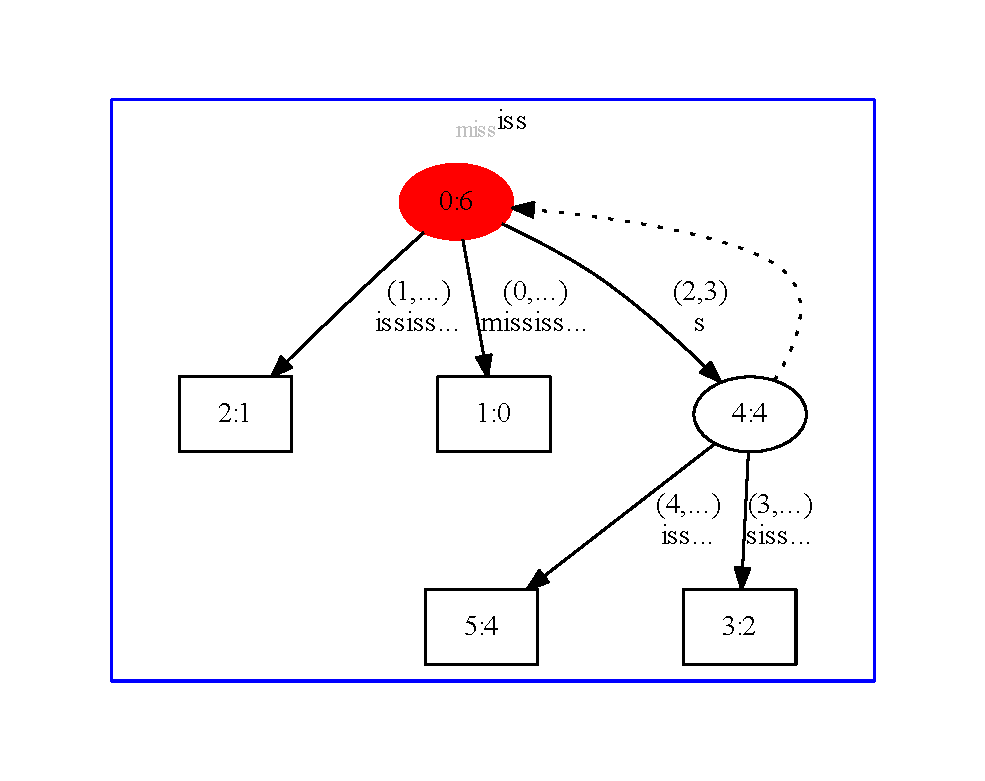
\includegraphics[keepaspectratio,trim=40pt 40pt 40pt 40pt,height=0.8\textheight,width=0.9\textwidth]{mississ.pdf}<7>
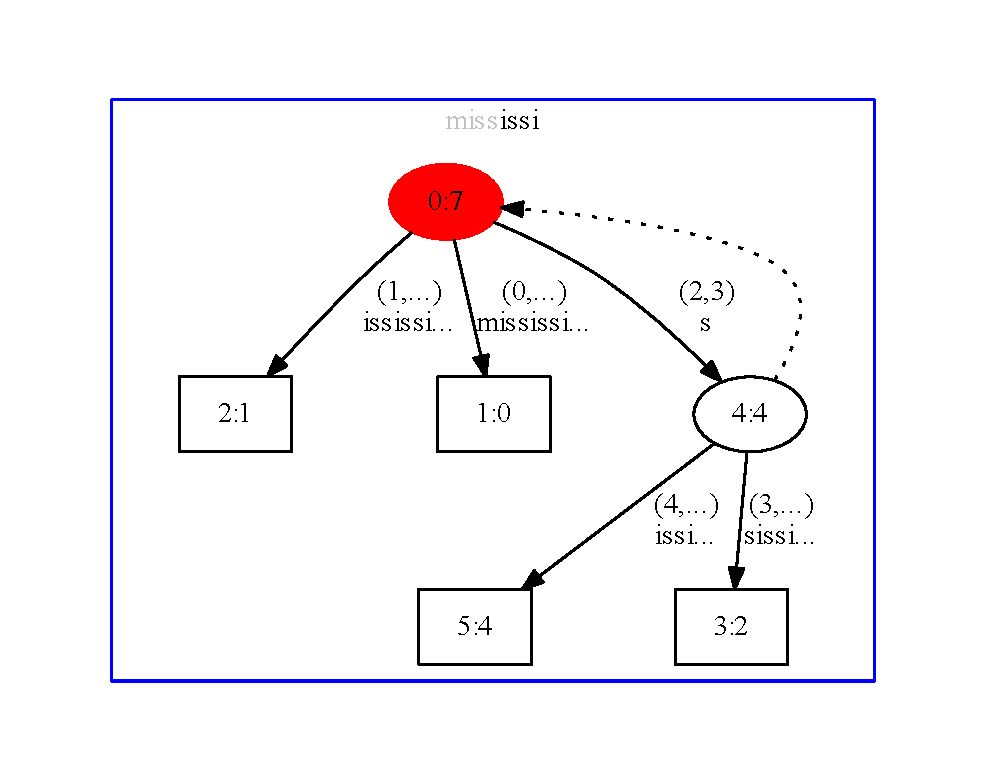
\includegraphics[keepaspectratio,trim=40pt 40pt 40pt 40pt,height=0.8\textheight,width=0.9\textwidth]{mississi.pdf}<8>
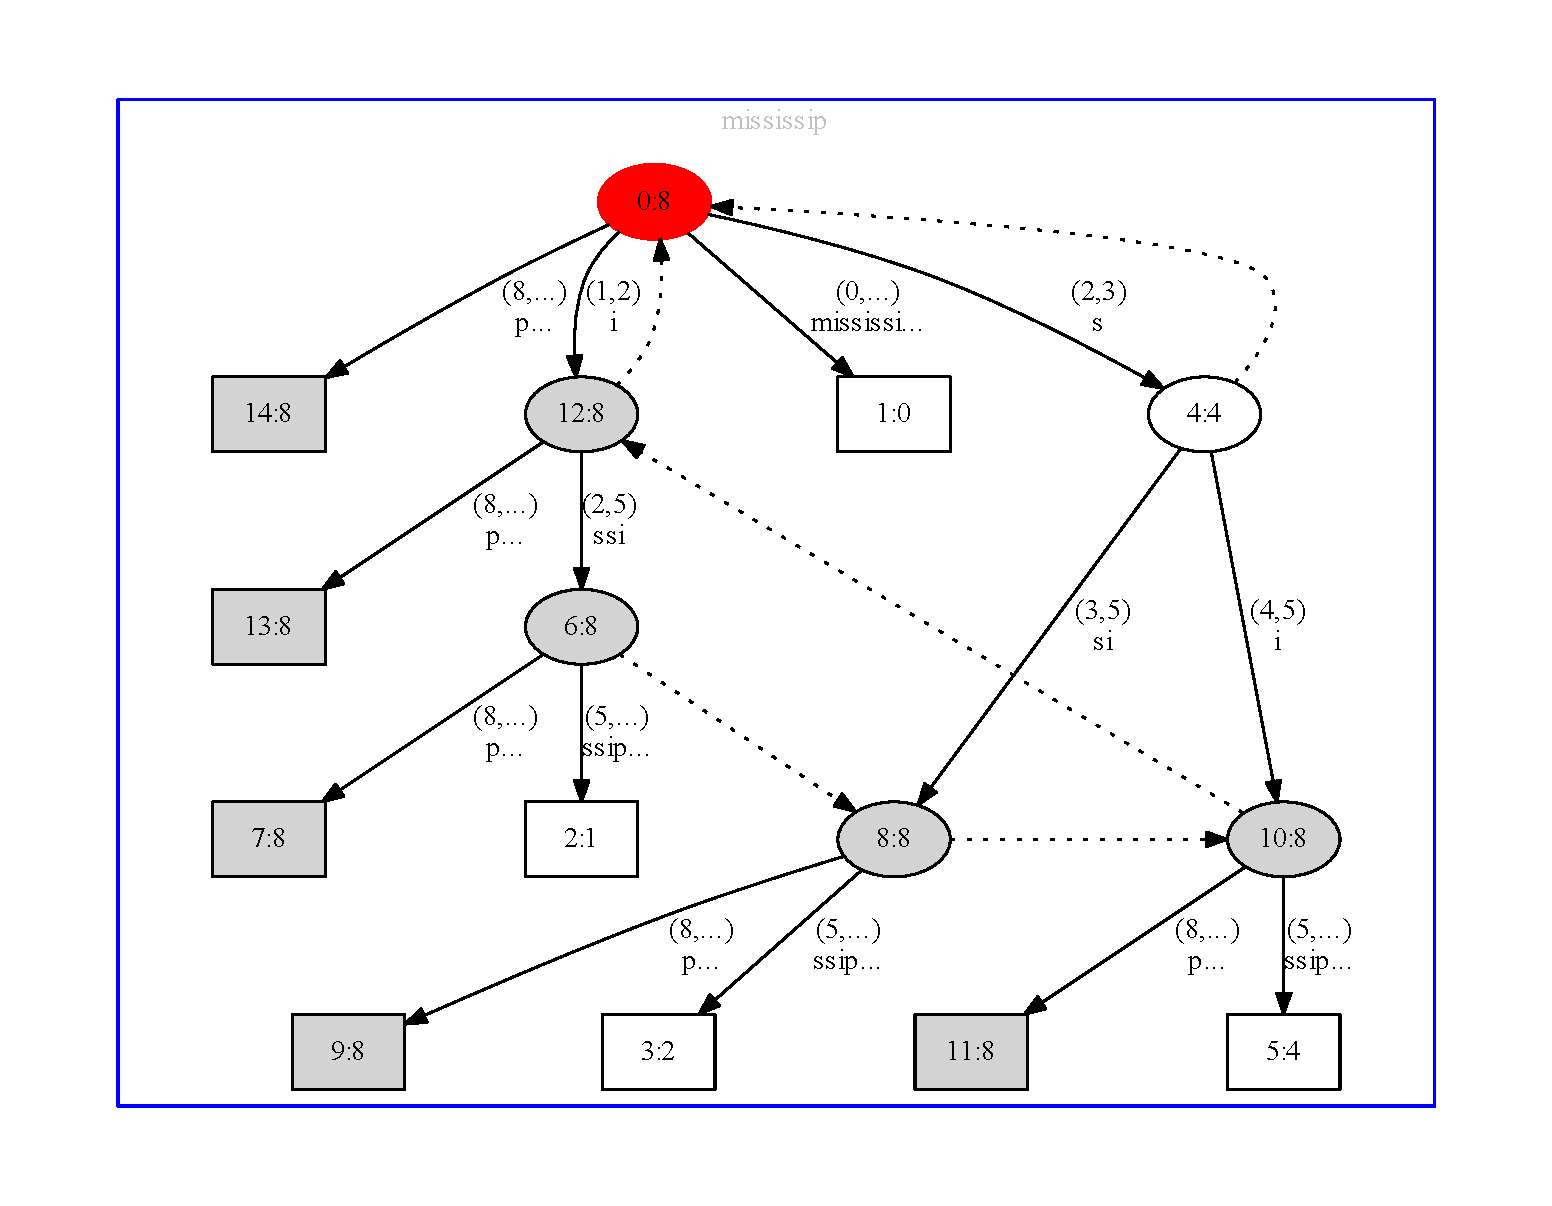
\includegraphics[keepaspectratio,trim=40pt 40pt 40pt 40pt,height=0.8\textheight,width=0.9\textwidth]{mississip.pdf}<9>
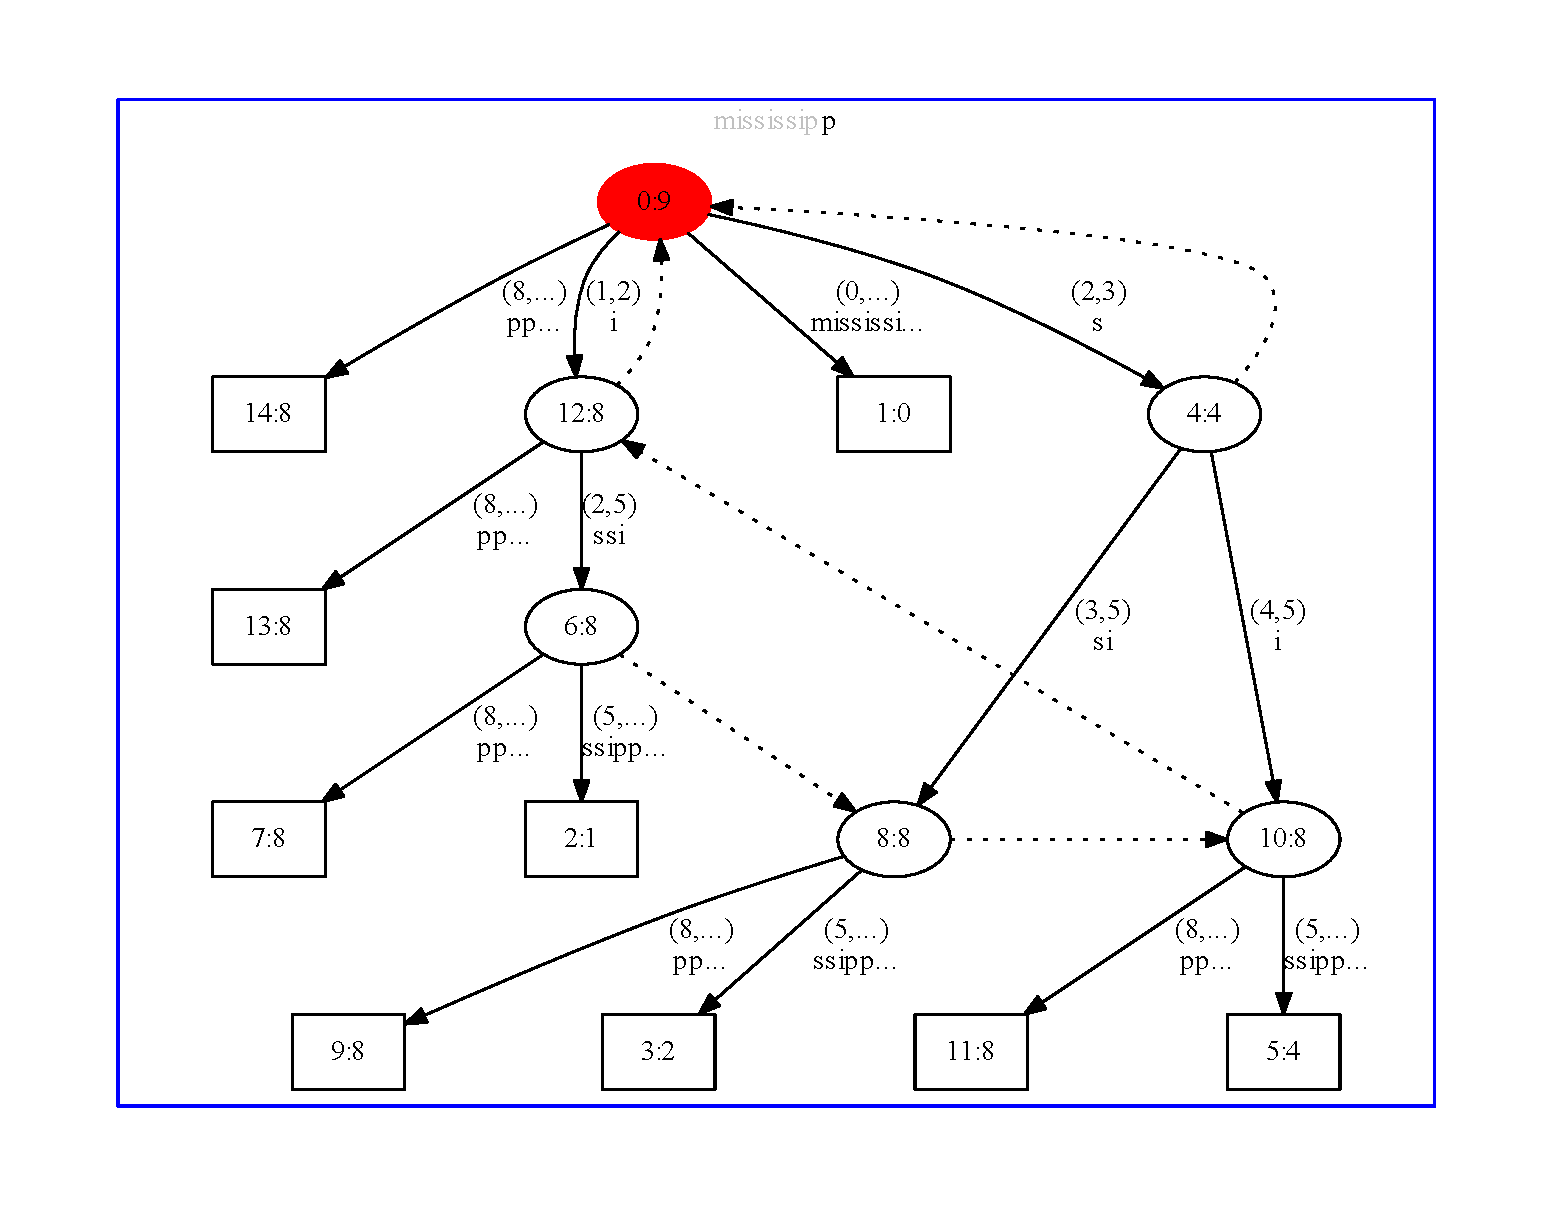
\includegraphics[keepaspectratio,trim=40pt 40pt 40pt 40pt,height=0.8\textheight,width=0.9\textwidth]{mississipp.pdf}<10>
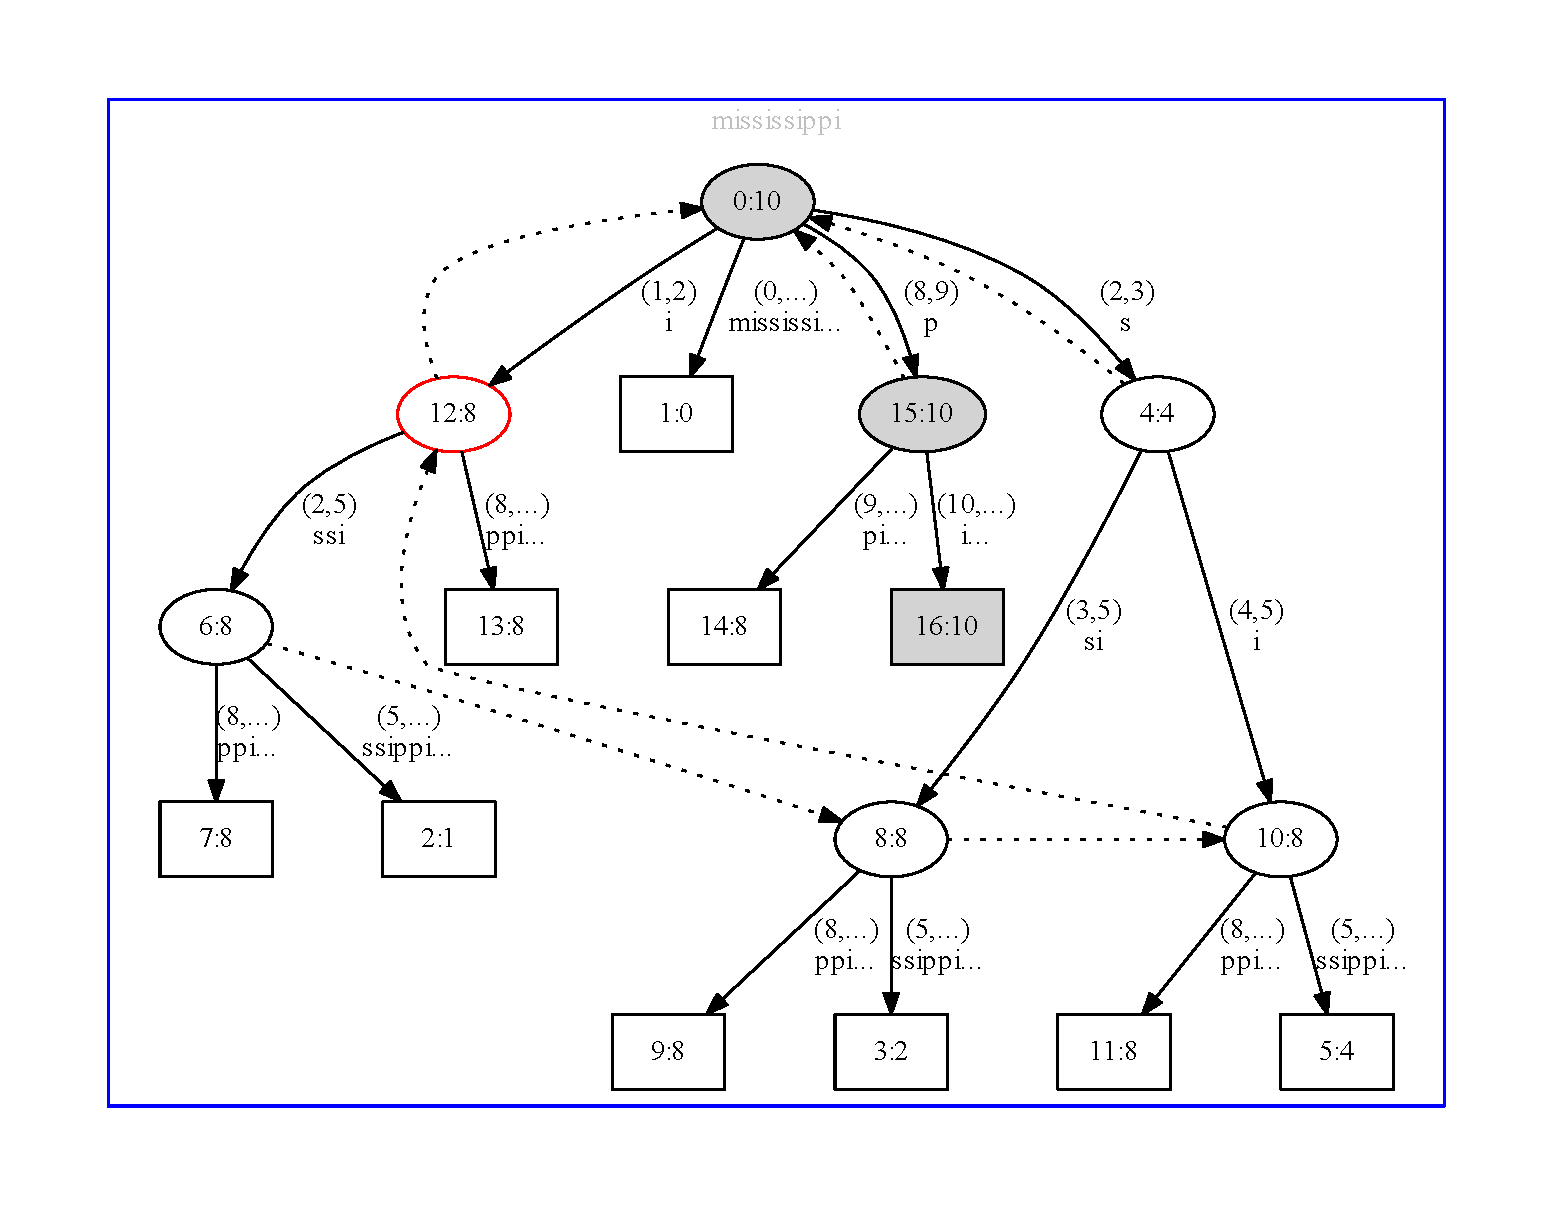
\includegraphics[keepaspectratio,trim=40pt 40pt 40pt 40pt,height=0.8\textheight,width=0.9\textwidth]{mississippi.pdf}<11>
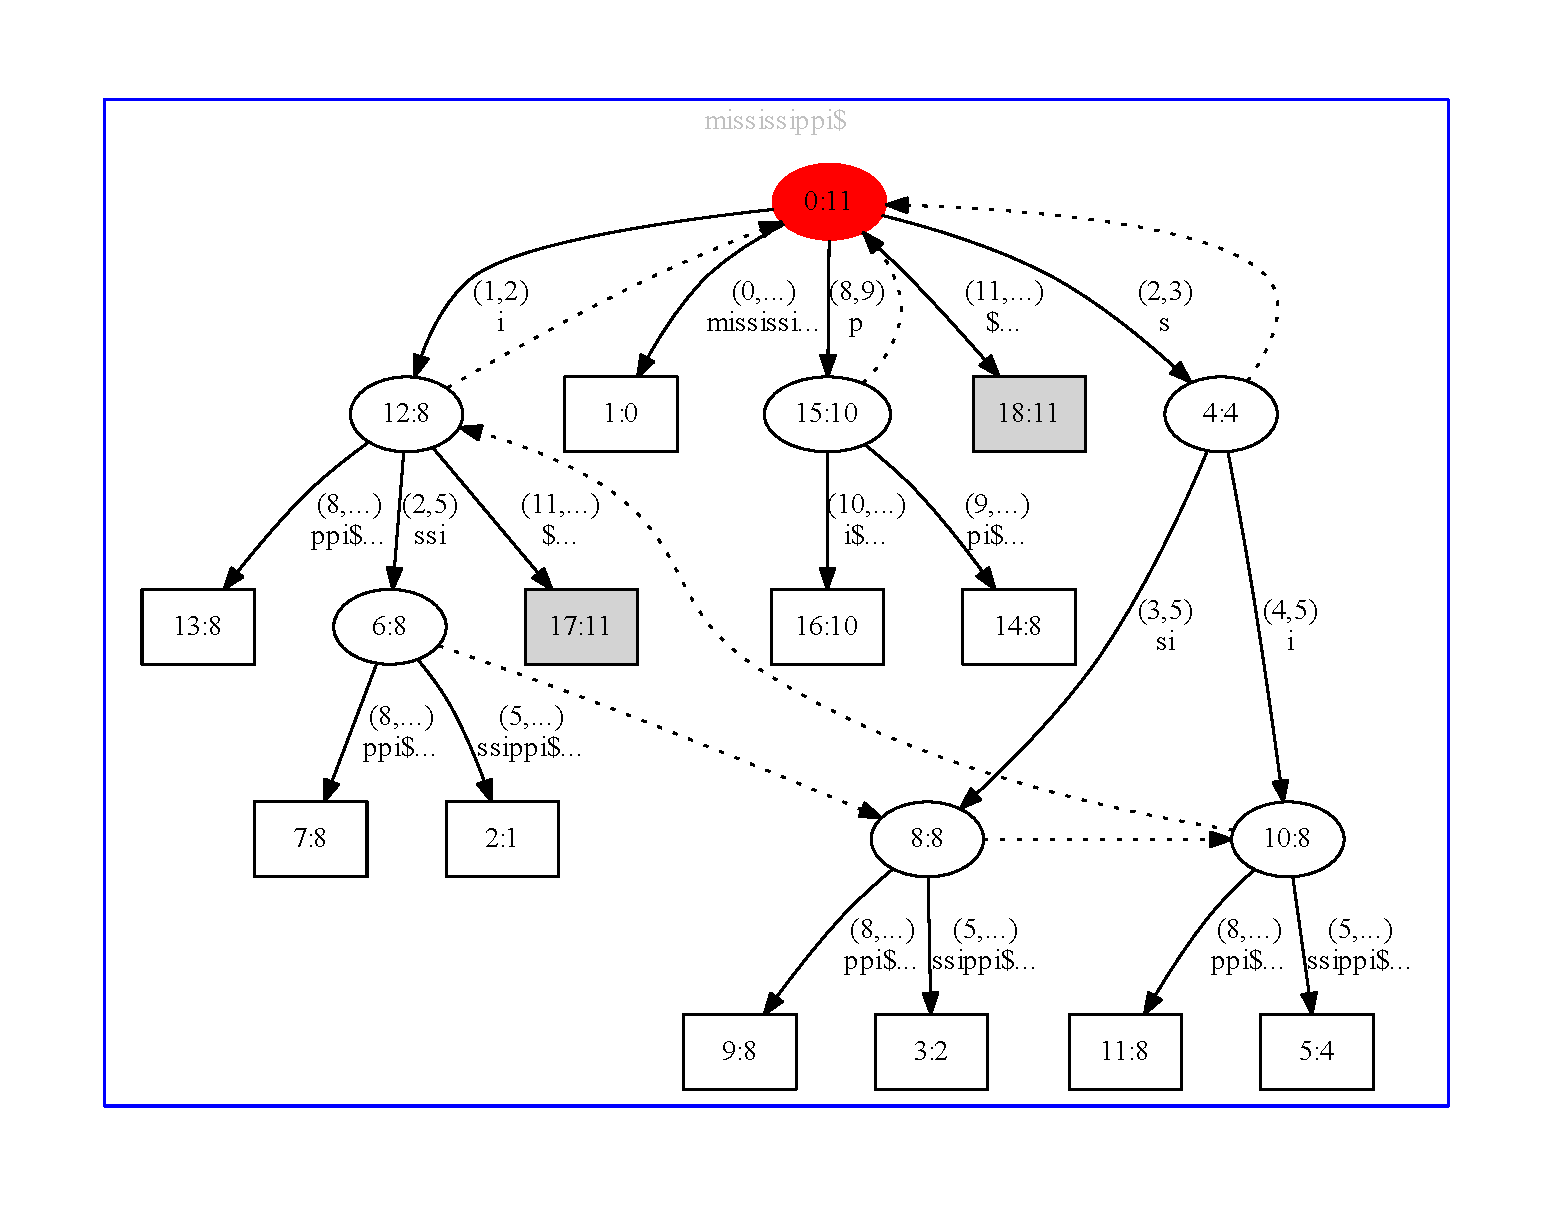
\includegraphics[keepaspectratio,trim=40pt 40pt 40pt 40pt,height=0.8\textheight,width=0.9\textwidth]{mississippi_.pdf}<12>
\end{overlayarea}
\end{frame}
%%%%%%%%%%%%%%%%%%%%%%%%%%%%%%%%%%%%%%%%%%%%%%%%%%%%%%%%%%%%%%%%%%%%%%%%%%%%%%%%
\begin{frame}{Time Complexity Analysis}
\begin{tikzpicture}[ node distance=0 cm,outer sep = 0pt,x=0.8cm, y=0.5cm]
\node at (0,1) {m};
\node at (0,2) {i};
\node at (0,3) {s};
\node at (0,4) {s};
\node at (0,5) {i};
\node at (0,6) {s};
\node at (0,7) {s};
\node at (0,8) {i};
\node at (0,9) {p};
\node at (0,10) {p};
\node at (0,11) {i};
\node at (0,12) {\$};

\node at (1,0) {m};
\node at (2,0) {i};
\node at (3,0) {s};
\node at (4,0) {s};
\node at (5,0) {i};
\node at (6,0) {s};
\node at (7,0) {s};
\node at (8,0) {i};
\node at (9,0) {p};
\node at (10,0) {p};
\node at (11,0) {i};
\node at (12,0) {\$};

\draw (1,1)--(1,2)--(2,2)--(2,3)--(3,3)--(3,4)--(3,5)--(4,5)--(4,6)--(4,7)--(4,8)--(4,9)--(5,9)--(6,9)--(7,9)--(8,9)--(9,9)--(9,10)--(9,11)--(10,11)--(11,11)--(11,12)--(12,12);
\end{tikzpicture}

Time complexity is $2 N = O(N)$ .
\end{frame}

%%%%%%%%%%%%%%%%%%%%%%%%%%%%%%%%%%%%%%%%%%%%%%%%%%%%%%%%%%%%%%%%%%%%%%%%%%%%%%%%
\begin{frame}[shrink=20]{Experiment -- English text}

%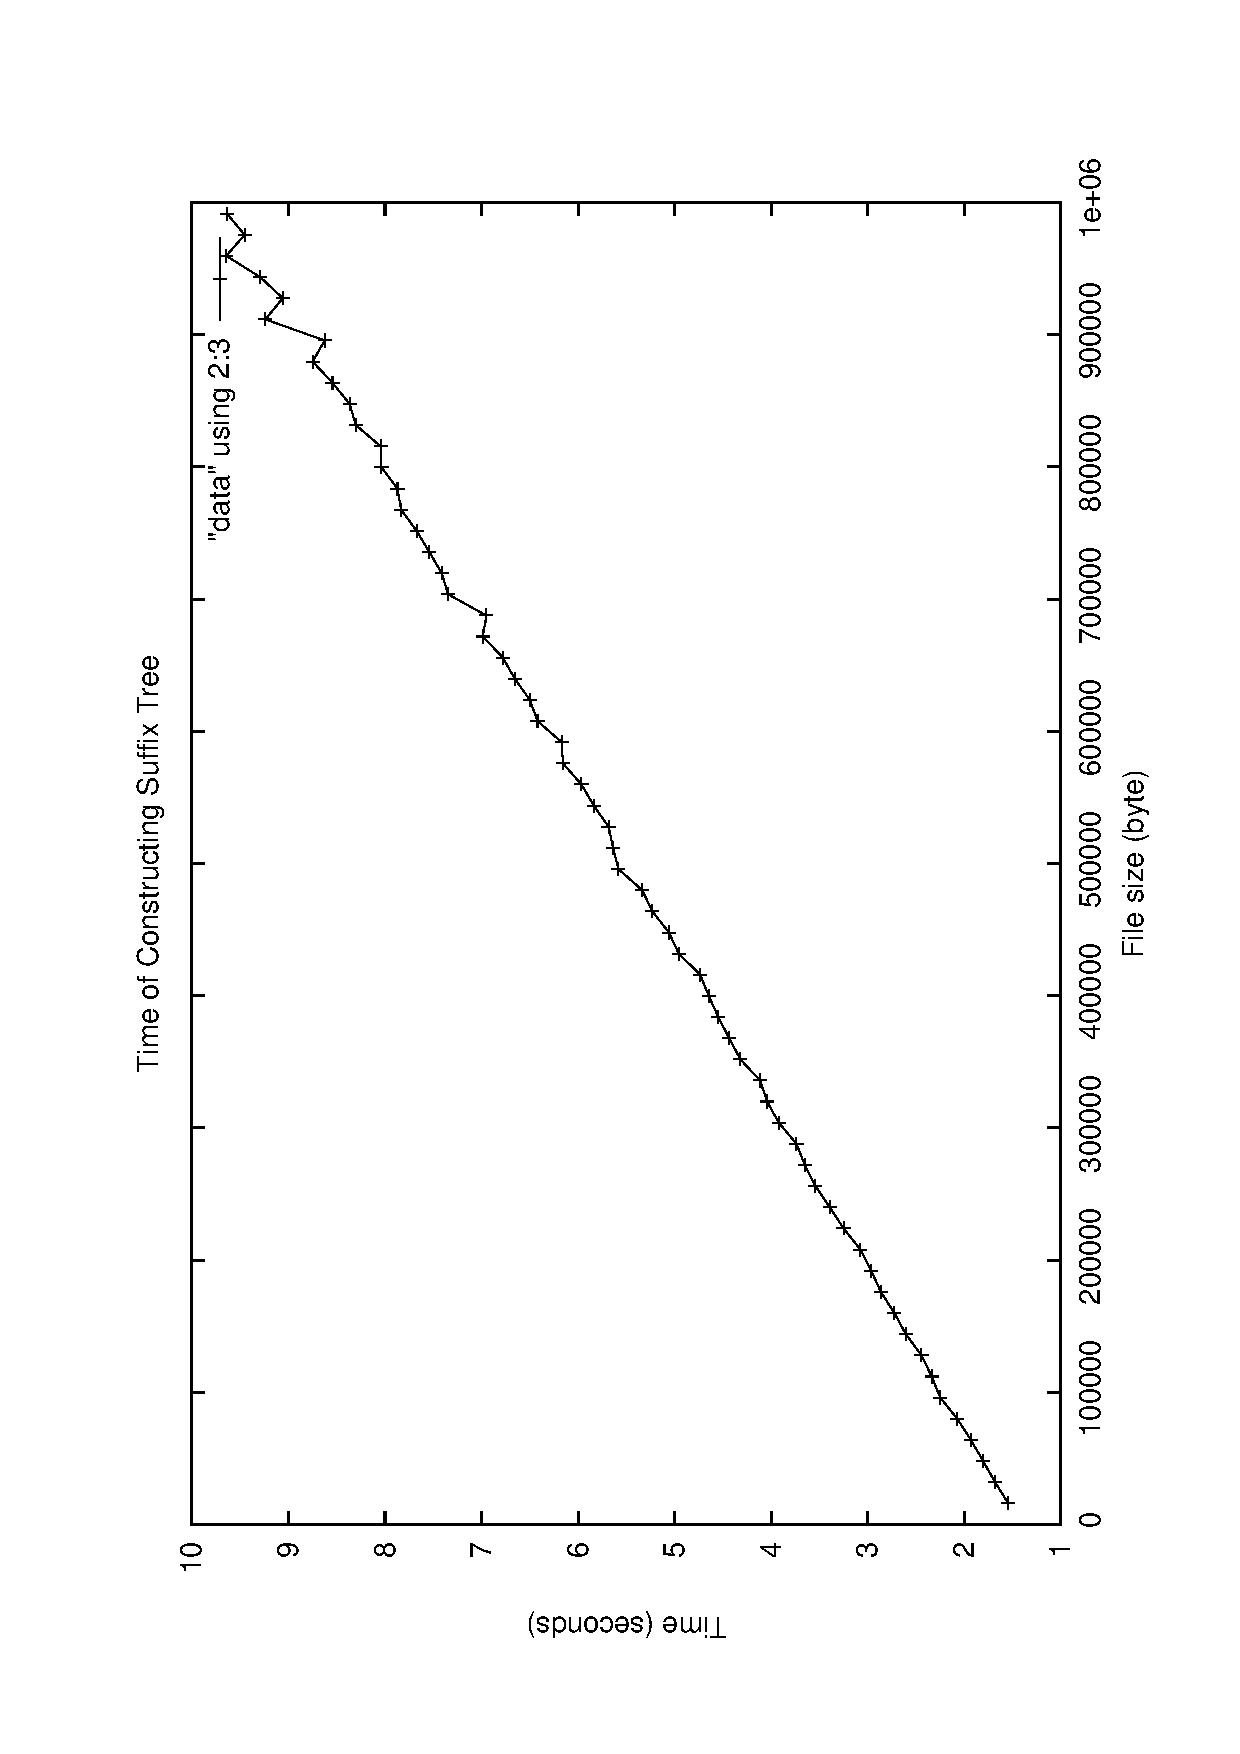
\includegraphics[angle=270,width=0.9\textwidth]{plot.fig}
%\documentclass{article}
%\usepackage{graphicx}

%\begin{document}
% GNUPLOT: LaTeX picture with Postscript
\begingroup
  \makeatletter
  \providecommand\color[2][]{%
    \GenericError{(gnuplot) \space\space\space\@spaces}{%
      Package color not loaded in conjunction with
      terminal option `colourtext'%
    }{See the gnuplot documentation for explanation.%
    }{Either use 'blacktext' in gnuplot or load the package
      color.sty in LaTeX.}%
    \renewcommand\color[2][]{}%
  }%
  \providecommand\includegraphics[2][]{%
    \GenericError{(gnuplot) \space\space\space\@spaces}{%
      Package graphicx or graphics not loaded%
    }{See the gnuplot documentation for explanation.%
    }{The gnuplot epslatex terminal needs graphicx.sty or graphics.sty.}%
    \renewcommand\includegraphics[2][]{}%
  }%
  \providecommand\rotatebox[2]{#2}%
  \@ifundefined{ifGPcolor}{%
    \newif\ifGPcolor
    \GPcolorfalse
  }{}%
  \@ifundefined{ifGPblacktext}{%
    \newif\ifGPblacktext
    \GPblacktexttrue
  }{}%
  % define a \g@addto@macro without @ in the name:
  \let\gplgaddtomacro\g@addto@macro
  % define empty templates for all commands taking text:
  \gdef\gplbacktext{}%
  \gdef\gplfronttext{}%
  \makeatother
  \ifGPblacktext
    % no textcolor at all
    \def\colorrgb#1{}%
    \def\colorgray#1{}%
  \else
    % gray or color?
    \ifGPcolor
      \def\colorrgb#1{\color[rgb]{#1}}%
      \def\colorgray#1{\color[gray]{#1}}%
      \expandafter\def\csname LTw\endcsname{\color{white}}%
      \expandafter\def\csname LTb\endcsname{\color{black}}%
      \expandafter\def\csname LTa\endcsname{\color{black}}%
      \expandafter\def\csname LT0\endcsname{\color[rgb]{1,0,0}}%
      \expandafter\def\csname LT1\endcsname{\color[rgb]{0,1,0}}%
      \expandafter\def\csname LT2\endcsname{\color[rgb]{0,0,1}}%
      \expandafter\def\csname LT3\endcsname{\color[rgb]{1,0,1}}%
      \expandafter\def\csname LT4\endcsname{\color[rgb]{0,1,1}}%
      \expandafter\def\csname LT5\endcsname{\color[rgb]{1,1,0}}%
      \expandafter\def\csname LT6\endcsname{\color[rgb]{0,0,0}}%
      \expandafter\def\csname LT7\endcsname{\color[rgb]{1,0.3,0}}%
      \expandafter\def\csname LT8\endcsname{\color[rgb]{0.5,0.5,0.5}}%
    \else
      % gray
      \def\colorrgb#1{\color{black}}%
      \def\colorgray#1{\color[gray]{#1}}%
      \expandafter\def\csname LTw\endcsname{\color{white}}%
      \expandafter\def\csname LTb\endcsname{\color{black}}%
      \expandafter\def\csname LTa\endcsname{\color{black}}%
      \expandafter\def\csname LT0\endcsname{\color{black}}%
      \expandafter\def\csname LT1\endcsname{\color{black}}%
      \expandafter\def\csname LT2\endcsname{\color{black}}%
      \expandafter\def\csname LT3\endcsname{\color{black}}%
      \expandafter\def\csname LT4\endcsname{\color{black}}%
      \expandafter\def\csname LT5\endcsname{\color{black}}%
      \expandafter\def\csname LT6\endcsname{\color{black}}%
      \expandafter\def\csname LT7\endcsname{\color{black}}%
      \expandafter\def\csname LT8\endcsname{\color{black}}%
    \fi
  \fi
  \setlength{\unitlength}{0.0500bp}%
  \begin{picture}(7200.00,5040.00)%
    \gplgaddtomacro\gplbacktext{%
      \csname LTb\endcsname%
      \put(814,704){\makebox(0,0)[r]{\strut{} 0}}%
      \put(814,1213){\makebox(0,0)[r]{\strut{} 2}}%
      \put(814,1722){\makebox(0,0)[r]{\strut{} 4}}%
      \put(814,2231){\makebox(0,0)[r]{\strut{} 6}}%
      \put(814,2740){\makebox(0,0)[r]{\strut{} 8}}%
      \put(814,3248){\makebox(0,0)[r]{\strut{} 10}}%
      \put(814,3757){\makebox(0,0)[r]{\strut{} 12}}%
      \put(814,4266){\makebox(0,0)[r]{\strut{} 14}}%
      \put(814,4775){\makebox(0,0)[r]{\strut{} 16}}%
      \put(946,484){\makebox(0,0){\strut{} 0}}%
      \put(1783,484){\makebox(0,0){\strut{} 20000}}%
      \put(2619,484){\makebox(0,0){\strut{} 40000}}%
      \put(3456,484){\makebox(0,0){\strut{} 60000}}%
      \put(4293,484){\makebox(0,0){\strut{} 80000}}%
      \put(5130,484){\makebox(0,0){\strut{} 100000}}%
      \put(5966,484){\makebox(0,0){\strut{} 120000}}%
      \put(6803,484){\makebox(0,0){\strut{} 140000}}%
      \put(176,2739){\rotatebox{-270}{\makebox(0,0){\strut{}Construction Time (sec.)}}}%
      \put(3874,154){\makebox(0,0){\strut{}File size (byte)}}%
    }%
    \gplgaddtomacro\gplfronttext{%
      \csname LTb\endcsname%
      \put(5816,4602){\makebox(0,0)[r]{\strut{}"data" using 1:3}}%
    }%
    \gplbacktext
    \put(0,0){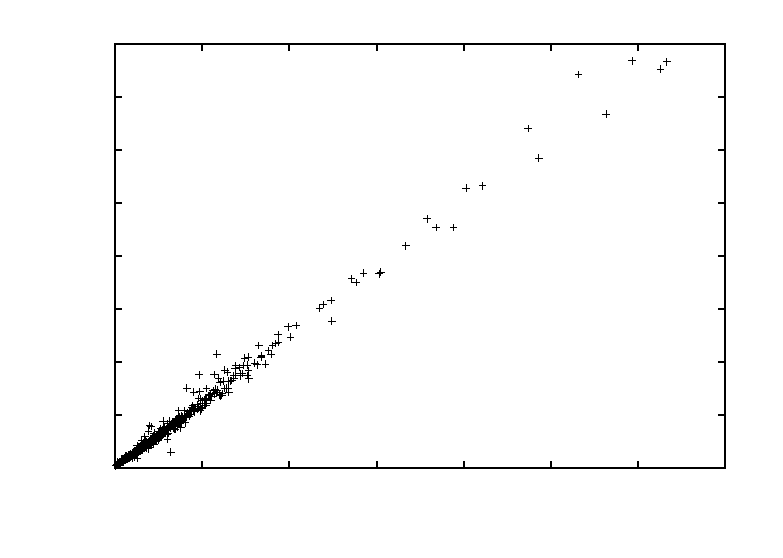
\includegraphics{plot}}%
    \gplfronttext
  \end{picture}%
\endgroup
%\end{document}

\end{frame}
%%%%%%%%%%%%%%%%%%%%%%%%%%%%%%%%%%%%%%%%%%%%%%%%%%%%%%%%%%%%%%%%%%%%%%%%%%%%%%%%

\end{document}
